%%%%%%%%%%%%%%%%%%%%%%%%%%%%%%%%%%%%%%%%%
% Masters/Doctoral Thesis 
% LaTeX Template
%
% This template was downloaded from:
% http://www.LaTeXTemplates.com
%
% Version 2.x major modifications by:
% Vel (vel@latextemplates.com)
%
% This template is based on a template by:
% Steve Gunn (http://users.ecs.soton.ac.uk/srg/softwaretools/document/templates/)
% Sunil Patel (http://www.sunilpatel.co.uk/thesis-template/)
%
% Template license:
% CC BY-NC-SA 3.0 (http://creativecommons.org/licenses/by-nc-sa/3.0/)
%
%%%%%%%%%%%%%%%%%%%%%%%%%%%%%%%%%%%%%%%%%

%----------------------------------------------------------------------------------------
%	PACKAGES AND OTHER DOCUMENT CONFIGURATIONS
%----------------------------------------------------------------------------------------

\documentclass[
11pt, % The default document font size, options: 10pt, 11pt, 12pt
%oneside, % Two side (alternating margins) for binding by default, uncomment to switch to one side
english, % ngerman for German
singlespacing, % Single line spacing, alternatives: onehalfspacing or doublespacing
%draft, % Uncomment to enable draft mode (no pictures, no links, overfull hboxes indicated)
%nolistspacing, % If the document is onehalfspacing or doublespacing, uncomment this to set spacing in lists to single
%liststotoc, % Uncomment to add the list of figures/tables/etc to the table of contents
%toctotoc, % Uncomment to add the main table of contents to the table of contents
%parskip, % Uncomment to add space between paragraphs
%nohyperref, % Uncomment to not load the hyperref package
headsepline, % Uncomment to get a line under the header
%chapterinoneline, % Uncomment to place the chapter title next to the number on one line
%consistentlayout, % Uncomment to change the layout of the declaration, abstract and acknowledgements pages to match the default layout
]{MastersDoctoralThesis} % The class file specifying the document structure

\usepackage{physics}
\usepackage{float}
\usepackage{braket}
\usepackage{amsmath}
\usepackage[utf8]{inputenc} % Required for inputting international characters
\usepackage[T1]{fontenc} % Output font encoding for international characters

\usepackage{mathpazo} % Use the Palatino font by default

\usepackage{biblatex}
% THEOREMS AND DEFINITIONS
\usepackage{amsthm}
% Definition
\theoremstyle{definition}
\newtheorem{definition}{Definition}[section]
%Remark
\theoremstyle{remark}
\newtheorem*{remark}{Remark}
%Theorem
\theoremstyle{theorem}
\newtheorem{theorem}{Theorem}[section]
\newtheorem{lemma}[theorem]{Lemma}
%Corollary
\theoremstyle{corollary}
\newtheorem{corollary}{Corollary}[theorem]

\addbibresource{references.bib} % The filename of the bibliography

\usepackage[autostyle=true]{csquotes} % Required to generate language-dependent quotes in the bibliography
\usepackage{hyperref}
\usepackage{tikz}
%----------------------------------------------------------------------------------------
%	MARGIN SETTINGS
%----------------------------------------------------------------------------------------

\geometry{
	paper=a4paper, % Change to letterpaper for US letter
	inner=2.0cm, % Inner margin 2.5
	outer=3.0cm, % Outer margin 3.8
	bindingoffset=.5cm, % Binding offset
	top=1.5cm, % Top margin
	bottom=1.5cm, % Bottom margin
	%showframe, % Uncomment to show how the type block is set on the page
}
\captionsetup{justification=raggedright,singlelinecheck=false}
%----------------------------------------------------------------------------------------
%	THESIS INFORMATION
%----------------------------------------------------------------------------------------

\thesistitle{Adiabatic Quantum Computing in Unit Commitment Problems in Electrical Power Flow} % Your thesis title, this is used in the title and abstract, print it elsewhere with \ttitle
\supervisor{Dr. Álvaro Díaz Fernández\\
Dr. Oriol Raventós Morera} % Your supervisor's name, this is used in the title page, print it elsewhere with \supname
\examiner{} % Your examiner's name, this is not currently used anywhere in the template, print it elsewhere with \examname
\degree{Master in Quantum Computing} % Your degree name, this is used in the title page and abstract, print it elsewhere with \degreename
\author{Sergio López Baños} % Your name, this is used in the title page and abstract, print it elsewhere with \authorname
\addresses{} % Your address, this is not currently used anywhere in the template, print it elsewhere with \addressname

\subject{Quantum Computing} % Your subject area, this is not currently used anywhere in the template, print it elsewhere with \subjectname
\keywords{} % Keywords for your thesis, this is not currently used anywhere in the template, print it elsewhere with \keywordnames
\university{\href{https://www.nebrija.com}{Nebrija University}} % Your university's name and URL, this is used in the title page and abstract, print it elsewhere with \univname
\department{\href{https://www.dlr.de/}{DLR - Deutsches Zentrum
für Luft- und Raumfahrt}} % Your department's name and URL, this is used in the title page and abstract, print it elsewhere with \deptname
\group{\href{https://www.dlr.de/ve/en/desktopdefault.aspx/tabid-12472/21440_read-49440/}{Institute of Networked Energy Systems}} % Your research group's name and URL, this is used in the title page, print it elsewhere with \groupname
\faculty{\href{https://www.dlr.de/}{Research Center}} % Your faculty's name and URL, this is used in the title page and abstract, print it elsewhere with \facname

\AtBeginDocument{
\hypersetup{pdftitle=\ttitle} % Set the PDF's title to your title
\hypersetup{pdfauthor=\authorname} % Set the PDF's author to your name
\hypersetup{pdfkeywords=\keywordnames} % Set the PDF's keywords to your keywords
}

\begin{document}

\frontmatter % Use roman page numbering style (i, ii, iii, iv...) for the pre-content pages

\pagestyle{plain} % Default to the plain heading style until the thesis style is called for the body content

%----------------------------------------------------------------------------------------
%	TITLE PAGE
%----------------------------------------------------------------------------------------

\begin{titlepage}
\begin{center}

%\vspace*{.06\textheight}

\includegraphics[scale=0.5]{logos/Nebrija.jpeg}
%{\scshape\LARGE \univname\par}\vspace{1.5cm} % University name
%\textsc{\Large Master Thesis}\\[0.5cm] % Thesis type

\HRule \\[0.4cm] % Horizontal line
{\huge \bfseries \ttitle\par}\vspace{0.4cm} % Thesis title
\HRule \\[1.5cm] % Horizontal line
 
\begin{minipage}[t]{0.4\textwidth}
\begin{flushleft} \large
\emph{\textbf{Author:}}\\
{\authorname} % Author name - remove the \href bracket to remove the link
\end{flushleft}
\end{minipage}
\begin{minipage}[t]{0.4\textwidth}
\begin{flushright} \large
\emph{\textbf{Supervisors:}} \\
{\supname} % Supervisor name - remove the \href bracket to remove the link  
\end{flushright}
\end{minipage}\\[3cm]
 
\vfill

\large \textit{A thesis submitted in fulfillment of the requirements \\ for the degree of \degreename \\ at Nebrija University.}\\[0.3cm] % University requirement text
\textit{The thesis was carried out in}\\[0.4cm]
\groupname\\\deptname\\[1cm] % Research group name and department name
\vfill
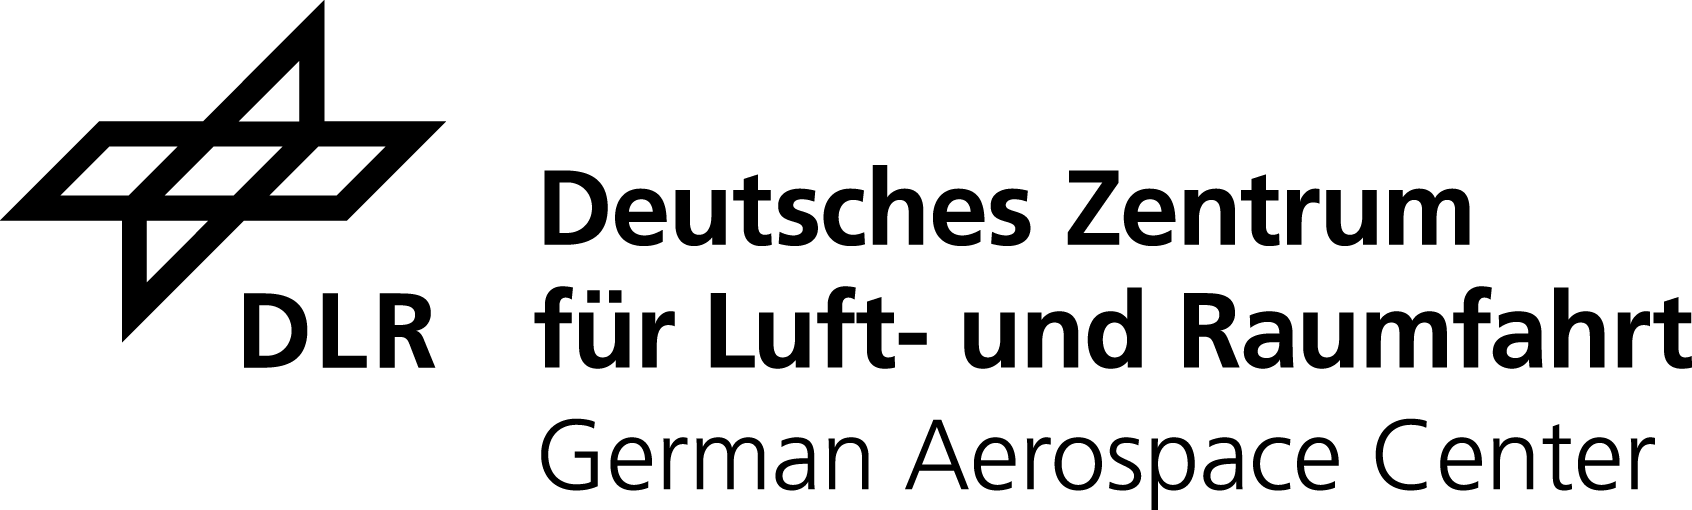
\includegraphics[scale=0.65]{logos/DLR_Logo_EN_schwarz.png} % University/department logo - uncomment to place it

%{\large \today}\\[4cm] % Date 
\vfill
\end{center}
\end{titlepage}

%----------------------------------------------------------------------------------------
%	DECLARATION PAGE
%----------------------------------------------------------------------------------------

\begin{declaration}
\addchaptertocentry{\authorshipname} % Add the declaration to the table of contents
\noindent I, \authorname, declare that this thesis titled, \enquote{\ttitle} and the work presented in it are my own. I confirm that:

\begin{itemize} 
\item This work was done wholly or mainly while in candidature for a research degree at this University.
\item Where any part of this thesis has previously been submitted for a degree or any other qualification at this University or any other institution, this has been clearly stated.
\item Where I have consulted the published work of others, this is always clearly attributed.
\item Where I have quoted from the work of others, the source is always given. With the exception of such quotations, this thesis is entirely my own work.
\item I have acknowledged all main sources of help.
\item Where the thesis is based on work done by myself jointly with others, I have made clear exactly what was done by others and what I have contributed myself.
\end{itemize}
 
\noindent Signed:\\
\rule[0.5em]{25em}{0.5pt} % This prints a line for the signature
 
\noindent Date:\\
\rule[0.5em]{25em}{0.5pt} % This prints a line to write the date
\end{declaration}

\cleardoublepage

%----------------------------------------------------------------------------------------
%	QUOTATION PAGE
%----------------------------------------------------------------------------------------

\vspace*{0.2\textheight}

\noindent\enquote{\itshape Thanks to my solid academic training, today I can write hundreds of words on virtually any topic without possessing a shred of information, which is how I got a good job in journalism.}\bigbreak

\hfill Dave Barry

%----------------------------------------------------------------------------------------
%	ABSTRACT PAGE
%----------------------------------------------------------------------------------------

\begin{abstract}
\addchaptertocentry{\abstractname} % Add the abstract to the table of contents
The Thesis Abstract is written here (and usually kept to just this page). The page is kept centered vertically so can expand into the blank space above the title too\ldots
\end{abstract}

%----------------------------------------------------------------------------------------
%	ACKNOWLEDGEMENTS
%----------------------------------------------------------------------------------------

\begin{acknowledgements}
\addchaptertocentry{\acknowledgementname} % Add the acknowledgements to the table of contents
The acknowledgments and the people to thank go here, don't forget to include your project advisor\ldots
\end{acknowledgements}

%----------------------------------------------------------------------------------------
%	LIST OF CONTENTS/FIGURES/TABLES PAGES
%----------------------------------------------------------------------------------------

\tableofcontents % Prints the main table of contents

\listoffigures % Prints the list of figures

\listoftables % Prints the list of tables

%----------------------------------------------------------------------------------------
%	ABBREVIATIONS
%----------------------------------------------------------------------------------------

\begin{abbreviations}{ll} % Include a list of abbreviations (a table of two columns)

\textbf{HPC} & \textbf{H}igh \textbf{P}erformance \textbf{C}omputing\\
\textbf{QUBO} & \textbf{Q}uadratic \textbf{U}nconstrained \textbf{B}inary \textbf{O}ptimization\\
\textbf{SA} & \textbf{S}imulated \textbf{A}nnealing \\
\textbf{QA} & \textbf{Q}uantum \textbf{A}nnealing \\
\end{abbreviations}

%----------------------------------------------------------------------------------------
%	PHYSICAL CONSTANTS/OTHER DEFINITIONS
%----------------------------------------------------------------------------------------

\begin{constants}{lr@{${}={}$}l} % The list of physical constants is a three column table

% The \SI{}{} command is provided by the siunitx package, see its documentation for instructions on how to use it

Speed of Light & $c_{0}$ & \SI{2.99792458e8}{\meter\per\second} (exact)\\
%Constant Name & $Symbol$ & $Constant Value$ with units\\

\end{constants}

%----------------------------------------------------------------------------------------
%	SYMBOLS
%----------------------------------------------------------------------------------------

\begin{symbols}{lll} % Include a list of Symbols (a three column table)

$a$ & distance & \si{\meter} \\
$P$ & power & \si{\watt} (\si{\joule\per\second}) \\
%Symbol & Name & Unit \\

\addlinespace % Gap to separate the Roman symbols from the Greek

$\omega$ & angular frequency & \si{\radian} \\

\end{symbols}

%----------------------------------------------------------------------------------------
%	DEDICATION
%----------------------------------------------------------------------------------------

\dedicatory{For/Dedicated to/To my\ldots} 

%----------------------------------------------------------------------------------------
%	THESIS CONTENT - CHAPTERS
%----------------------------------------------------------------------------------------

\mainmatter % Begin numeric (1,2,3...) page numbering

\pagestyle{thesis} % Return the page headers back to the "thesis" style

% Include the chapters of the thesis as separate files from the Chapters folder
% Uncomment the lines as you write the chapters

% Chapter Template

\chapter{Introduction} % Main chapter title

\label{Chapter1} % Change X to a consecutive number; for referencing this chapter elsewhere, use \ref{ChapterX}

%----------------------------------------------------------------------------------------
%	SECTION 1
%----------------------------------------------------------------------------------------
%
% Statment of the problem + Motivation
%
Quantum computing is a new paradigm of computation whose importance is growing not only because of its promising speed-up over classical computers in some problems, such as combinatorial optimization problems, but also due to the fact that we are building transistors in a scale where quantum effects are starting to become relevant. Combinatorial optimization problems are common among industry albeit more research needs to be done to get insight about how quantum computing could help to solve industry challenges. There is already a large industry research in finance\,\cite{Herman2022AFinance}, route planning\,\cite{Tambunan2022QuantumSegment} and life sciences, among others. The research on applications of quantum computing to the energy sector has just began in the last years. There are only a few active research projects, like Q-Grid by e-On\,\cite{Fernandez-Campoamor2021CommunityAnnealing} or EnerQuant by Fraunhofer. The goal of this work to contribute to this field of research.
\begin{figure}[H]
  \begin{center}
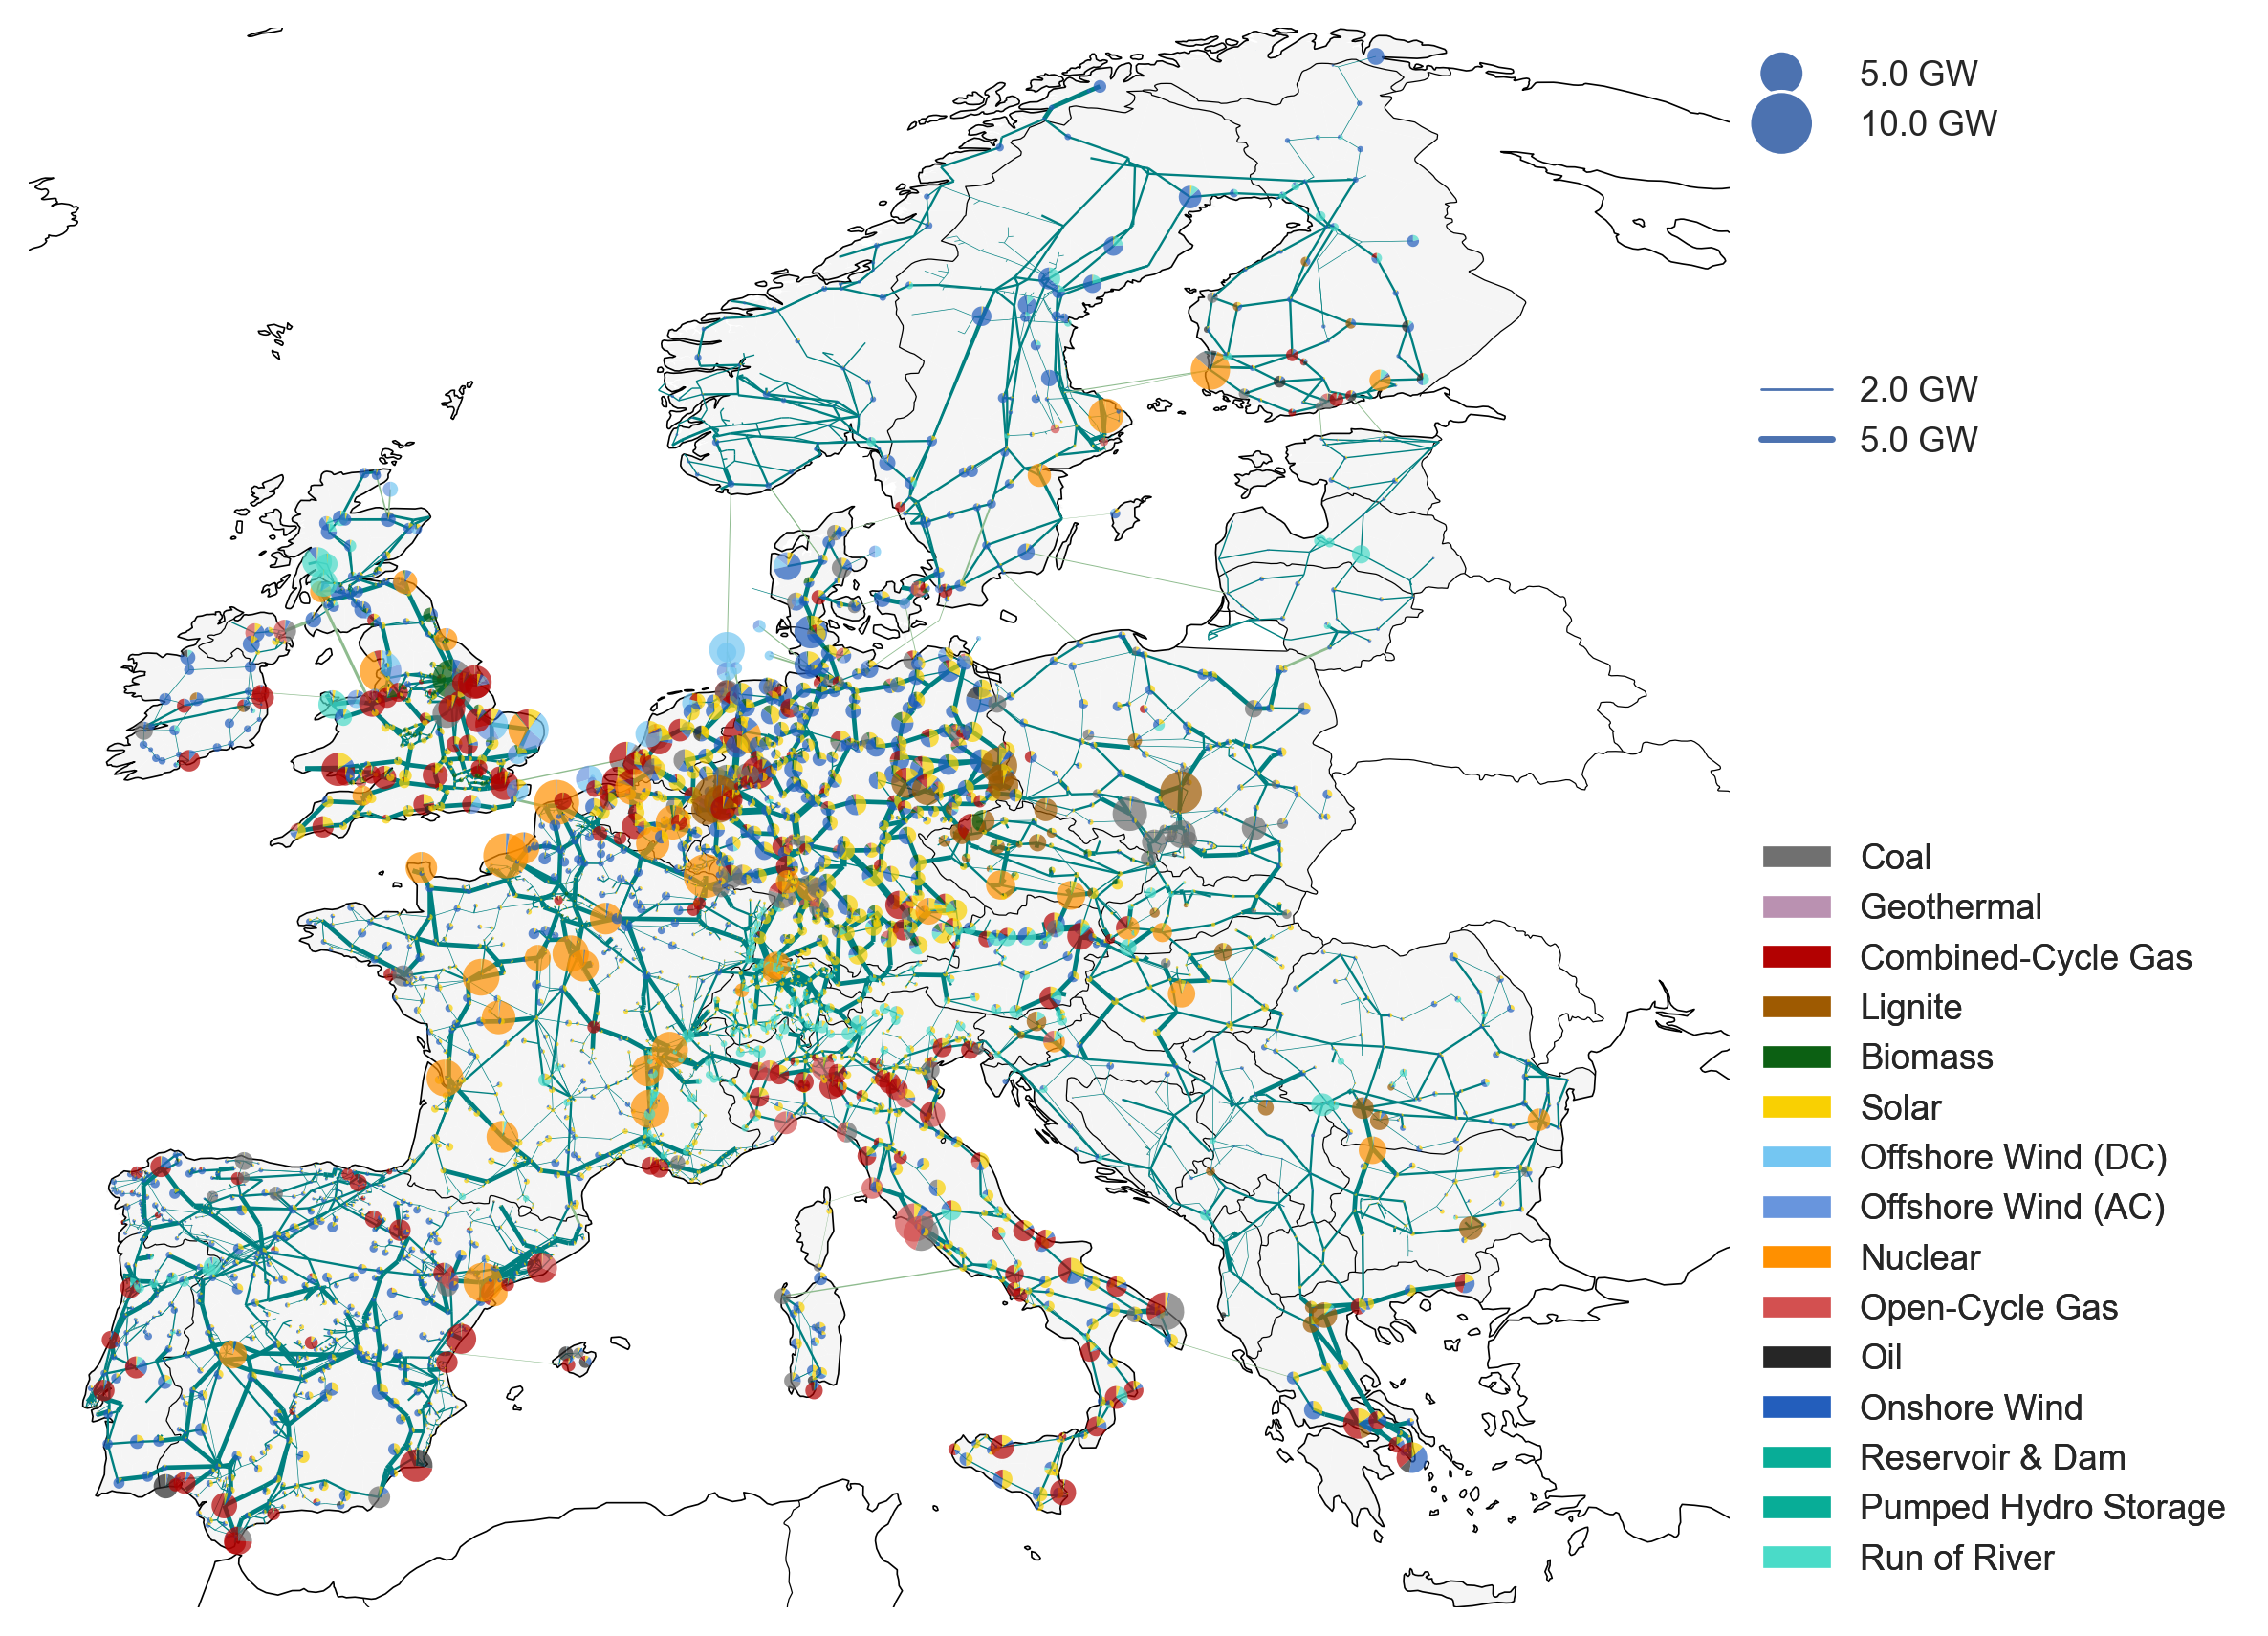
\includegraphics[width=0.85\textwidth]{Figures/Europe-Grid.png}
  \end{center}
  \caption{Clustered European transmission network model obtained from PyPSA-EUR\,\cite{PyPSA-Eur:PyPSA-Eur}.}
\end{figure}
Energy system models are getting larger and more complex due to the integration of decentralized weather-dependent renewable energy sources, intermittent loads, sector coupling and the increase of storage components. For instance, the renewable energy produced by the integration of solar panels in dwellings is intended to be integrated to the grid if consumers are not using it. However, the grid infrastructure is not evolving accordingly to the new energy paradigm. As a consequence, energy from private sources cannot be added to the grid, which implies the efficiency of solar panels has to be decreased or the excess of energy has to be discarded. An accurate expansion planning would solve these problems by redirecting the excess of energy to where it is required or by storing it so that it can be used later, e.g., to charge an electric car. In this way, the energy would be efficiently distributed and energy companies could offer better prices to their consumers while safeguarding the environment by reducing their carbon footprints. Furthermore, an increment of the quantity of detailed data about energy consumption -- smart meters -- would extend the spatial and temporal resolution, i.e., the grid status of a region, so that better managing and expansion planning decisions can be made in order to satisfy the customer demand efficiently.\\\\ 
The problem we tackle in the present work is called \textit{transmission expansion planning} (TEP) problem, which is a \textit{mixed-integer linear programming} (MILP) problem with NP complexity, that aims at finding the optimal way to expand the capacity and connections of an energy system. Currently, the scope and granularity of the model are reduced using clustering algorithms. For this reason, any computational time reduction will have substantial implications in closing the granularity gap between what the current models can solve and the desired resolution needed by energy system operators.\\\\
Quantum computers are the candidates to solve NP-hard problems such as MILP, by making the complexity of the problem scale polynomically as the systems size grows. Concretely, quantum analog computers are special-purpose quantum computers specialised in solving combinatorial optimization problems. The size of quantum analog computers that is the number of qubits of the system is greater than the general purpose quantum computers such as the ones from IBM that are based in the successive applications of quantum gates, such as the recently released Osprey quantum processor with 433 qubits.
%
% Objectives of my thesis
%
Although quantum computers are improving every few years they are not mature enough for solving many real-world problems where the number of variables scales exponentially. Also, we have to take into account that quantum computers are hugely affected by the environmental conditions\footnote{John Preskill called the current state of quantum technology as the Noisy Intermediate-Scale Quantum era, or NISQ for short\,\cite{Preskill2018}.} -- Noisy Intermediate-Scale Quantum (NISQ) era --, meaning that there will be errors during an algorithm execution, which implies that the execution time has to be short enough so that it does not exceed quantum decoherence. Because of the current maturity of quantum computers, hybrid quantum-classical approaches are required to tackle real-world problems\,\cite{Callison2022HybridBeyond}. The hybrid approach combines classical solvers and cutting-edge classical algorithms with quantum solvers that add the speed-up where it is possible.\\\\
A benchmark of how a TEP problem can be scaled up until current quantum solvers are not able to find a solution is provided among with a scheme to decompose a large TEP problem into a small enough master problem that can be addressed by a quantum computer and a sub-problem addressed by a classical computer. \\\\
% Structure of the thesis
%
The present work is structured as follows. Chapter\,\ref{Chapter2} guides through the foundations of adiabatic quantum computing. Chapter\,\ref{Chapter3} describes Benders' decomposition techniques in the field of quantum computing. Chapter\,\ref{Chapter4} solves a transmission expansion problem by starting with a small network solved by a pure quantum annealer and ending up with a bigger network that requires from hybrid solvers. Conclusions and outlook are drawn in Chapter\,\ref{Chapter5}.

%% Chapter 2

\chapter{Adiabatic Quantum Computing} % Main chapter title

\label{Chapter2} % For referencing the chapter elsewhere, use \ref{Chapter1} 
In the present chapter, we show a paradigm of quantum computation known as \textit{adiabatic quantum computing} (AQC), see Ref. \cite{Farhi2000QuantumEvolution}. We start by sketching the rough idea of the adiabatic theorem to finally derive a formal proof of it. We also expose one application of AQC to solve \textit{quadratic unconstrained binary optimization} (QUBO) problems, known as \textit{quantum annealing} (QA), see Ref. \cite{Kadowaki1998QuantumModel}.

%%%%%%%%%%%%%%%%%%%%%%%%%%%%%%%%%%%%%%%%%%%%%%%%%%%%%%%%%%%%%%%%%%%%%%%%%%%%%%%%%%%%%%%%%%%%%%%%%%%%%%%%%%
%     1.1 ADIABATIC APPROXIMATION
%%%%%%%%%%%%%%%%%%%%%%%%%%%%%%%%%%%%%%%%%%%%%%%%%%%%%%%%%%%%%%%%%%%%%%%%%%%%%%%%%%%%%%%%%%%%%%%%%%%%%%%%%%
\section{The Adiabatic Theorem}
Quoting Sarandy and Lidar\,\cite{Sarandy2005AdiabaticSystems},
\begin{displayquote}
\textit{The theorem posits, roughly, that if a state is an instantaneous eigenstate of a sufficiently slowly varying Hamiltonian at one time, then it will remain an eigenstate at later times, while its eigenenergy evolves continuously.}
\end{displayquote}
\subsection{The adiabatic protocol}
We need to construct an initial Hamiltonian $\mathcal{H}(t=0) = \mathcal{H}_{i}$ whose ground state is known and whose time evolution, $t \in \left[0,T\right]$ -- where $T$ is the total evolution time -- leads to a Hamiltonian $\mathcal{H}(t=T) = \mathcal{H}_{f}$ that encodes the solution to our problem. Mathematically we can write a linear schedule between the initial and target Hamiltonian,
\begin{equation}
\label{eq:Htime}
    \mathcal{H}(t) = \left(1-\frac{t}{T}\right)\mathcal{H}_{i} + \left(\frac{t}{T} \right)\mathcal{H}_{f}.
\end{equation}
The adiabatic theorem guarantees that if we start with an initial Hamiltonian $\mathcal{H}_{i}$ in a given eigenspace and the evolution is carried out sufficiently slowly -- in further sections we demonstrate what slowly means in detail -- then we end up in the equivalent eigenspace of the final Hamiltonian $\mathcal{H}_{f}$. \\\\
The adiabatic protocol can be summarized as follows:
\begin{itemize}
    \item \textbf{Step 1 (Mapping):} Map the problem into a Hamiltonian $\mathcal{H}_{f}$. Typically, the problem is encoded in the ground state.
    \item \textbf{Step 2 (Initialise $\mathcal{H}_{i}$):} Initialise the system in the ground state of a Hamiltonian $\mathcal{H}_{i}$, easy to compute and to experimentally prepare. For instance, the ground state of $\mathcal{H} = - \sum_{i}^{n}\hat{\sigma}_{i}^{x}$ is the eigenvector $\ket{+}^{\otimes n}$.
    \item \textbf{Step 3 (Adiabatic Theorem):} Slowly evolve the system from $H_{i}$ to $H_{f}$. The adiabatic theorem guarantees that, under certain conditions that will be explained later, the system will end up in the ground state of $H_{f}$.
    \item \textbf{Step 4 (Measure):} Measure the eigenstate of $H_{f}$. The result encodes a solution to our problem.
\end{itemize}
Notice that we wrote in the last step that the result of the measurement provides "a solution" not "the solution". This is because there are two possibilities for a finite-dimensional Hamiltonian:
\begin{itemize}
    \item \textbf{Non-degenerate Hamiltonian:} We start with an initial Hamiltonian $\mathcal{H}_{i}$ in its ground eigenstate $\ket{g(t=0)}$ and end up in the equivalent eigenstate -- ground state -- of the final Hamiltonian $\mathcal{H}_{f}$ where the eigenvalue is $E_{g}(t=T)$ and the eigenvector is\\
    $\ket{g(t=T)}$.
    \item \textbf{Degenerate Hamiltonian:} We start with an initial Hamiltonian $\mathcal{H}_{i}$ in its ground eigen-\\
    space spanned by $\{\ket{g^{i}(t=0)}\}_{i \in \left[1,d\right]}$, where $d$ is the degeneracy of the ground state, and end up in the equivalent eigenspace of the final Hamiltonian $\mathcal{H}_{f}$ with eigenvalue $E_{g}(t=T)$.
\end{itemize}
Intuitively, one can think that a problem can have multiple configurations that lead to the same minimum eigenvalue.
%%%%%%%%%%%%%%%%%%%%%%%%%%%%%%%%%%%%%%%%%%%%%%%%%%%%%%%%%%%%%%
\subsection{The Adiabatic Theorem: A First Approach}
We now provide a simple argument to build intuition into the adiabatic theorem. The next section will be devoted to a formal proof. In order to continue, let us define the following dimensionless variable
\begin{equation}
    s \equiv \frac{t}{T}\, , \quad s \in [0,1].
\end{equation}
In what follows, we consider an $n$-qubit system with a discrete and non-degenerate spectrum. A state of that system can be written as a linear combination of the instantaneous eigenstates of the Hamiltonian $\ket{\psi(s)} = \sum_{i}c_{i}(s)\ket{i(s)}$ as function of $s$. Its evolution is given by the time-dependent Schrödinger equation, see Appx.\,\ref{AppendixA},
\begin{equation}
\label{eq:GeneralEv}
    i\hbar \ket{\dot{\psi}(s)} = \mathcal{H}(s) \ket{\psi(s)}.
\end{equation}
In general, Eq.\,\eqref{eq:GeneralEv} represents a system of coupled differential equations for the evolution of the state $\ket{\psi(s)}$ which has a non-trivial solution. However, we can re-write the Hamiltonian in diagonal form using the change-of-basis matrix $U(s)$,
\begin{equation}
    \mathcal{H}_{d}(s) = U^{-1}(s)\mathcal{H}(s)U(s) = \begin{bmatrix}
           \lambda_{0} & 0 & \hdots & 0 \\
           0 &  \ddots & & \vdots \\
           \vdots &   & \ddots & 0 \\
           0 & \hdots & 0 & \lambda_{2^{n-1}}
         \end{bmatrix}.
\end{equation}
We also define $\ket{\psi_{d}(s)} = U^{-1}(s)\ket{\psi(s)}$ as the state we get after applying the inverse transformation $U^{-1}(s)$ to the state $\ket{\psi(s)}$. Using the identity $\mathbb{I} = U(s)U^{-1}(s)$ and multiplying both sides of Eq.\,\eqref{eq:GeneralEv} by $U^{-1}(s)$ yields
\begin{equation}
     i\hbar U^{-1}(s) \frac{\partial \left(U(s)U^{-1}(s)\ket{\psi(s)}\right)}{\partial s} = U^{-1}(s)\mathcal{H}(s) \left(U(s)U^{-1}(s)\right)\ket{\psi(s)}.
\end{equation}
Rearranging terms
\begin{equation}
     i\hbar U^{-1}(s) \frac{\partial U(s)}{\partial s}\ket{\psi_{d}(s)} + i\hbar  \frac{\partial \ket{\psi_{d}(s)}}{\partial s}= \mathcal{H}_{d}(s)\ket{\psi_{d}(s)}.
\end{equation}
If we assume $\mathcal{H}(s)$ varies slowly, then it is reasonable that $U(s)$ varies slowly as well, $\dot{U}(s) \simeq 0$, which implies
\begin{equation}
    i\hbar  \frac{\partial \ket{\psi_{d}(s)}}{\partial s} \simeq \mathcal{H}_{d}(s)\ket{\psi_{d}(s)}.
\end{equation}
Now, the evolution of the state $\ket{\psi_{d}(s)}$ is led by a diagonal Hamiltonian $\mathcal{H}_{d}(s)$ so we have a set of uncoupled differential equations for each amplitude component of the state $\ket{\psi_{d}(s)}$. Furthermore, if the state of the system $\ket{\psi_{d}(s)}$ is an eigenstate of the Hamiltonian $\ket{n(s)}$, then the evolution of our system is conducted inside the eigenspace generated by $\ket{n(s)}$.\\\\
To sum up, under a general evolution such as Eq.\,\eqref{eq:GeneralEv} we get, in general, a system of coupled differential equations, but if the adiabatic approximation is satisfied, this evolution is led by a diagonal Hamiltonian, i.e., we get a system of uncoupled differential equations. Graphically, this means the eigenenergies $E_{n}(s)$ of the Hamiltonian's instantaneous eigenstates $\ket{n(s)}$ do not cross.
\begin{figure}[H]
\centering
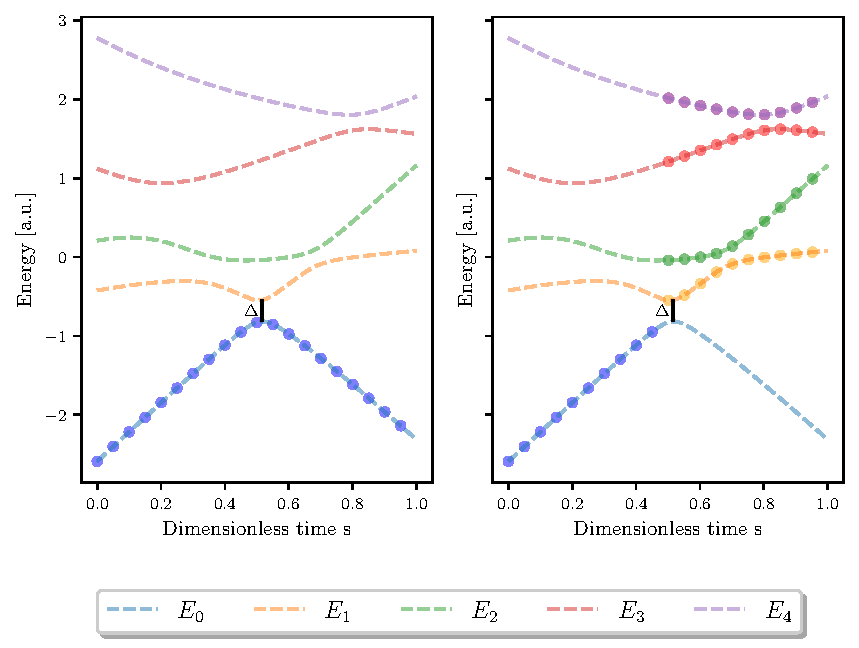
\includegraphics[width=\textwidth]{Figures/Eigenenergies.pdf}
    \caption{Eigenenergies of a random Hamiltonian as function of dimensionless time $s=t/T$. The dots indicate the state of the system at each point in time. \textbf{Left}: when adiabatic conditions are fulfilled, i.e., if the evolution is carried out sufficiently slowly, then our system evolves continuously in time along the ground state. \textbf{Right}: when the evolution is carried out not fulfilling the adiabatic conditions, it could happen that we end up in a different eigenstate if our system absorbs enough energy to jump to next level over the evolution, something that is more likely to happen close to the minimum gap in the minimum gap $\Delta$. If that happens we would end up in a different eigenstate of the target Hamiltonian which does not encode the optimal solution.}
    \label{fig:Eigenenergies}
\end{figure}
\newpage
Quoting Goldstone \textit{et al.}\,\cite{Farhi2000QuantumEvolution},
\begin{displayquote}
\textit{...if the gap between the two lowest levels, $E_{1} - E_{0}$, is strictly greater than zero for all $0 \leq t \leq T$, then}
\end{displayquote}
\begin{equation}
    \lim_{T\longrightarrow \infty} | \braket{g(t=T) | \psi(t=T)}| = 1.
\end{equation}
Equivalently, the probability of being in the ground state, $\ket{g(t=T)}$, of the target Hamiltonian $\mathcal{H}_{f}$ at the end of evolution is 1 if and only if the total time required for the evolution is infinite. Otherwise, the probability of being in the ground state is
\begin{equation}
    || \braket{g(t=T) | \psi(t=T)}||^{2} = 1 - \epsilon^{2},
\end{equation}
where $|\epsilon| \leq 1$ takes into account the error due to the adiabatic approximation, $\dot{U}(s) \simeq 0$.
%%%%%%%%%%%%%%%%%%%%%%%%%%%%%%%%%%%%%%%%%%%%%%%%%%%%%%%%%%%%%%%%%%%%%%%%%%%%%%%%%%%%%%%%%%%%%%%%%%%%%%%%%%
%     1.2 ADIABATIC THEOREM
%%%%%%%%%%%%%%%%%%%%%%%%%%%%%%%%%%%%%%%%%%%%%%%%%%%%%%%%%%%%%%%%%%%%%%%%%%%%%%%%%%%%%%%%%%%%%%%%%%%%%%%%%%
\subsection{The Adiabatic Theorem: A Formal Derivation}
We start by writing down the Schrödinger equation
\begin{equation}
    i\hbar \frac{\partial \ket{\psi(t)}}{\partial t} = \mathcal{H}(t)\ket{\psi(t)}.
\end{equation}
We assume that the instantaneous spectrum of $\mathcal{H}(t)$ is discrete and non-degenerate
\begin{equation}
\label{eq:Hamiltonian}
    \mathcal{H}(t) \ket{n(t)} = E_{n}(t)\ket{n(t)},
\end{equation}
where $\ket{n(t)}$ are the instantaneous eigenstates of the Hamiltonian and $E_{n}(t)$ are the eigenenergies labelled by $n$. Notice that we can label the eigenenergies with a single index because the spectrum is discrete and non-degenerate. For a discrete but degenerate spectrum, we would need an extra index to take into account the degeneracy of each state.\\\\
The eigenstates of the Hamiltonian form an orthonormal basis, so we can expand a given state in that basis
\begin{equation}
\label{eq: EigenvectorExpansion}
    \ket{\psi(t)} = \sum_{n}c_{n}(t)e^{i\theta_{n}(t)} \ket{n(t)},
\end{equation}
where
\begin{equation}
    \theta_{n}(t) = -\frac{1}{\hbar}\int_{0}^{t}E_{n}(t^{\prime})dt^{\prime},
\end{equation}
is the dynamic phase.\\
Substituting Eq.\,\eqref{eq: EigenvectorExpansion} into the Schrödinger equation yields
\begin{equation}
    \sum_{n}\left[\dot{c}_{n}(t)\ket{n(t)} + c_{n}(t)\ket{\dot{n}(t)}\right]e^{i\theta_{n}(t)} = 0.
\end{equation}
Multiplying by $\bra{m(t)}$ we get
\begin{equation}
\label{eq:Coefficients}
    \dot{c}_{m}(t) = - \sum_{n}c_{n}\braket{m(t)|\dot{n}(t)}e^{i\left(\theta_{n}(t) - \theta_{m}(t)\right)}.
\end{equation}
We need to re-write $\braket{m(t)|\dot{n}(t)}$ in terms of the Hamiltonian's derivative using Eq.\,\eqref{eq:Hamiltonian}. If we derive that expression with respect to time, we find
\begin{equation}
    \frac{\partial \mathcal{H}(t)}{\partial t}\ket{n(t)} + \mathcal{H}(t)\frac{\partial \ket{n(t)}}{\partial t} = \frac{\partial E_{n}(t)}{\partial t} \ket{n(t)} + E_{n}(t)\frac{\partial \ket{n(t)}}{\partial t}. 
\end{equation}
Multiplying the last expression by $\bra{m(t)}$, with $m\neq n$,
\begin{equation}
    \braket{m(t)|\frac{\partial\mathcal{H}(t)}{\partial t}|n(t)} + E_{m}(t)\braket{m(t)|\dot{n}(t)} = E_{n}(t)\braket{m(t)|\dot{n}(t)}.
\end{equation}
Finally,
\begin{equation}
    \braket{m(t)|\dot{n}(t)} = \frac{1}{E_{n}(t)-E_{m}(t)}\braket{m(t)|\frac{\partial \mathcal{H}(t)}{\partial t}|n(t)}.
\end{equation}
Substituting into Eq.\,\eqref{eq:Coefficients} and defining $g_{nm}(t)\equiv E_{n}(t) - E_{m}(t)$ as the energy difference as a function of time $t$ between the eigenstates $\ket{m(t)}$ and $\ket{n(t)}$ leads to
\begin{equation}
\label{eq:GeneralCoefficientsNoadiabaticApprox}
    \dot{c}_{m}(t) = -c_{m}(t) \braket{m(t)|\dot{m}(t)} - \sum_{n\neq m} c_{n}(t)\frac{\braket{m(t)|\dot{\mathcal{H}}(t)|n(t)}}{g_{nm}(t)}e^{i\left(\theta_{n}(t) - \theta_{m}(t)\right)}.
\end{equation}
Adiabatic evolution is ensured if the coefficients $c_{n}(t)$ evolve independently from each other, i.e., if their dynamical equations do not couple. Mathematically,
\begin{equation}
    \max_{0 \leq t \leq T} \abs{\frac{\braket{m(t)|\dot{\mathcal{H}}(t)|n(t)}}{g_{nm}(t)}} \ll \min_{0\leq t \leq T} \abs{g_{nm}(t)}
\end{equation}
where $T$ is the total evolution time.\\ 
Under the adiabatic approximation, the coupling term tends to zero, that is,
\begin{equation}
    \sum_{n\neq m} c_{n}\frac{\braket{m(t)|\dot{\mathcal{H}(t)}|n(t)}}{g_{nm}(t)}e^{i\left(\theta_{n}(t) - \theta_{m}(t)\right)} \to 0.
\end{equation}
Therefore, equation Eq.\,\eqref{eq:GeneralCoefficientsNoadiabaticApprox} turns into
\begin{equation}
    \dot{c}_{m}(t) = -c_{m}(t)\braket{m(t)|\dot{m}(t)},
\end{equation}
whose solution is
\begin{equation}
    c_{m}(t) = c_{m}(0)e^{i\gamma_{m}(t)},
\end{equation}
where
\begin{equation}
    \gamma_{m}(t) = i\int_{0}^{t}\braket{m(t^{\prime})|\dot{m}(t^{\prime})}dt^{\prime} \quad \gamma_{m}\in \mathbb{R},
\end{equation}
is the Berry's phase.
%%%%%%%%%%%%%%%%%%%%%%%%%%%%%%%%%%%%%%%%%%%%%%%%%%%%%%%%%%%%%%%%%%%%%%%%
%       TOTAL EVOLUTION TIME
%%%%%%%%%%%%%%%%%%%%%%%%%%%%%%%%%%%%%%%%%%%%%%%%%%%%%%%%%%%%%%%%%%%%%%%%
\subsection{Total Evolution Time T}
In previous sections, we stated that under a sufficiently slowly Hamiltonian evolution the adiabatic theorem is satisfied. In this section, we define what "slow" means by deriving an expression to estimate the total time $T$ required for the adiabatic evolution\,\cite{Sarandy2005AdiabaticSystems}. We also demonstrate that the total time not only depends on the energy gap between the ground state and the first excited state but also on the term $\braket{m(s)|d\mathcal{H}(s)/ds|n(s)}$.\\\\
We start by re-writing Eq.\,\eqref{eq:GeneralCoefficientsNoadiabaticApprox} in terms of the normalised time $s = \frac{t}{T}$ and Berry's phase.
\begin{equation}
    e^{i\gamma_{m}(sT)}\frac{1}{T}\frac{\partial }{\partial s}\left[c_{m}(sT)e^{-i\gamma_{m}(sT)}\right] = -\sum_{n\neq m} c_{n}(sT) \frac{\braket{m(sT)|\dot{\mathcal{H}}(sT)|n(sT)}}{g_{nm}(sT)}e^{-i\left(\theta_{n}(sT) - \theta_{m}(sT)\right)}
\end{equation}
Notice we have added two Berry's phases terms with opposite sign so they cancel out. Integrating the last equation and re-arranging terms leads to
\begin{equation}
\label{eq:Coeff}
    c_{m}(s)e^{-i\gamma_{m}(s)} = c_{m}(0) - \sum_{n\neq m}\int_{0}^{s} ds^{\prime}\frac{F_{nm}(s^{\prime})}{g_{nm}(s^{\prime})}e^{-iT\int_{0}^{s^{\prime}}ds^{\prime\prime}\left(g_{nm}(s^{\prime\prime})\right)}.
\end{equation}
This equation expresses the coefficient $c_{n}(s)$ in terms of its initial value $c_{n}(0)$ and a summation term that keeps the rest of coefficients $c_{m}(s)$ with $m\neq n$, where
\begin{equation}
\label{eq:Fnm}
    F_{nm}(s) = c_{n}(s)\braket{m(s)|\dot{\mathcal{H}}(s)|n(s)} e^{-i\gamma_{m}(s)}.
\end{equation}
We can express the integrand of Eq.\,\eqref{eq:Coeff} as a difference between two terms,
\begin{align}
\frac{F_{nm}(s^{\prime})}{g_{nm}(s^{\prime})} e^{-iT\int_{0}^{s^{\prime}}\left(ds^{\prime \prime}g_{nm}(s^{\prime\prime}) \right)}= \frac{i}{T}\Biggl[\frac{d}{ds^{\prime}}\left(\frac{F_{nm}(s^{\prime})}{g^{2}_{nm}(s^{\prime})}e^{-iT\int_{0}^{s^{\prime}}\left(ds^{\prime \prime}g_{nm}(s^{\prime\prime}) \right)}\right)\\
 - e^{-iT\int_{0}^{s^{\prime}}\left(ds^{\prime \prime}g_{nm}(s^{\prime\prime}) \right)} \frac{d}{ds^{\prime}}\left(\frac{F_{nm}(s^{\prime})}{g_{nm}(s^{\prime})}\right)\Biggr].
 \end{align}
 Substituting the previous result into Eq.\,\eqref{eq:Coeff} leads to
 \begin{equation}
 \begin{split}
      c_{m}(s)e^{-i\gamma_{m}(s)} & = c_{m}(0) + \frac{i}{T}\Biggr[\frac{F_{nm}(0)}{g^{2}_{nm}(0)} - \frac{F_{nm}(s)}{g^{2}_{nm}(s)}e^{-iT\int_{0}^{s}ds^{\prime}g_{nm}(s^{\prime \prime})} \\
      & + \int_{0}^{s}ds^{\prime} e^{-iT\int_{0}^{s^{\prime}}\left(ds^{\prime \prime}g_{nm}(s^{\prime\prime}) \right)} \cdot \frac{d}{ds^{\prime}}\left(\frac{F_{nm}(s^{\prime})}{g_{nm}(s^{\prime})}\right)\Biggr].
\end{split}
\end{equation}
 Assuming the energy gap does not vanish when $T \rightarrow \infty$ and that $d\{F_{nm}(s^{\prime})/g_{nm}^{2}(s^{\prime})\}/ds^{\prime}$ is integrable for all $s \in [0,1]$, the Riemann-Lebesgue lemma\,\cite{BrownChurchill} guarantees that the last integral vanishes in the limit $T \rightarrow \infty$. So
  \begin{align}
  \label{eq:cm}
     c_{m}(s)e^{-i\gamma_{m}(s)} = c_{m}(0) + \frac{i}{T}\left[\frac{F_{nm}(0)}{g^{2}_{nm}(0)} - \frac{F_{nm}(s)}{g^{2}_{nm}(s)}e^{-iT\int_{0}^{s}ds^{\prime}g_{nm}(s^{\prime \prime})}\right].
 \end{align}
 Under the adiabatic conditions there are not mixing terms, i.e., the coefficient $c_{n}(s)$ does not depend on the rest of coefficients. Mathematically,
\begin{equation}
    c_{m}(m) = c_{0}(s)e^{i\gamma_{m}(s)}.
\end{equation}
Therefore, we can simplify Eq.\,\eqref{eq:Fnm}
\begin{equation}
    F_{nm}(s) = c_{n}(0)\braket{m(s)|\dot{\mathcal{H}}|n(s)} e^{-i\left[\gamma_{m}(s) - \gamma_{n}(s)\right]}.
\end{equation}
 With that simplification, we can estimate the total time for an adiabatic evolution by imposing a condition that minimises the second term of Eq.\,\eqref{eq:cm}
 \begin{equation}
     T \gg \frac{F}{g^{2}},
 \end{equation}
 where
 \begin{align}
     &F = \max_{0 \leq s \leq 1} \left|c_{n}(0)\braket{m(s)|\frac{d\mathcal{H}(s)}{ds}| n(s)}\right| \\
     &g = \min_{0 \leq s \leq 1} |g_{nm}(s)|.
 \end{align}
%-------------------------------------------------------------------------------------
% QUANTUM ANNEALING
%---------------------------------------------------------------------------------------
\section{Quantum Annealing}
\textit{Quantum annealing} (QA) takes its name from a classical heuristic algorithm named s\textit{imulated annealing} (SA), see Appx.\,\ref{AppendixB}. It is a particularization of AQC where the Hamiltonian is the Ising's Hamiltonian
\begin{equation}
    \mathcal{H}(s) = -\sum_{ij}\mathcal{J}_{ij}\sigma_{i}^{z}\sigma_{j}^{z} - h\sum_{i}\sigma_{i}^{z}.
\end{equation}
Spin information is given by the eigenvalues of Pauli Z-operators $\sigma^{z}$, where the possibles outcomes are $\{-1,1\}$ corresponding to the eigenvectors $\{\ket{\uparrow},\ket{\downarrow}\}$, respectively.\\\\
We also need an initial Hamiltonian whose ground state is easy to compute and prepare, e.g.,
\begin{equation}
    \mathcal{H}(s) = -\sum_{i}^{n}\sigma_{i}^{x},
\end{equation}
with ground state $\ket{+}^{n}$. This ground state considers all the possible configurations of our systems with a uniform distribution.\\\\
The annealing schedule between these Hamiltonians is given by
\begin{equation}
    \mathcal{H}(s) = -\sum_{ij}\mathcal{J}_{ij}\sigma_{i}^{z}\sigma_{j}^{z} - h\sum_{i}\sigma_{i}^{z} - \Gamma(s)\sum_{i}\sigma_{i}^{x},
\end{equation}
where $\Gamma(s)\sum_{i}\sigma_{i}^{x}$ represents the quantum fluctuations -- single-spin flip -- and $\Gamma(s)$ plays the same role as temperature in SA. The way of controlling the quantum fluctuations depends on the hardware we are using. The hardware implementation and topology of the quantum computer we have used in the present work is discussed in Appx.\,\ref{AppendixC}.\\\\
Initially, at $s \rightarrow 0$, the dominating term is $\Gamma(s)\sum_{i}\sigma_{i}^{x}$ because $\Gamma(s)$ takes a large value, but at later times $s \rightarrow 1$, $\Gamma(s)$ takes a value close to zero so the dominating Hamiltonian is $\mathcal{H}(s) = -\sum_{ij}\mathcal{J}_{ij}\sigma_{i}^{z} - h\sum_{i}\sigma_{i}^{z}$ which is the Hamiltonian we are interested in, as it contains the solution to our problem encoded in the ground state.
%------------------------------------------------------------------
% Formlation of QUBO problems
%------------------------------------------------------------------
\subsection{Formulation of Quadratic Unconatrained Binary Optimization Problems}
\begin{definition}{\textit{Quadratic Unconstrained Binary Optimization} (QUBO)}
   A Quadratic unconstrained binary optimization problem can be written as
\begin{equation}
    \min_{\vec{x}}\vec{x}^{T}Q\vec{x},
\end{equation}
where $n$ is the total number of binary variables, $\vec{x}\in\{0,1\}^{n}$ are the binary variables of the problem and $Q$ is an $n\times n$ matrix whose entries encodes our problem.
\end{definition}
Notice that the Ising Hamiltonian uses the binary variables $s_{i} = \{-1,1\}$ but QUBO problems are formulated with the binary variables $x_{i} = \{0,1\}$. Both formulations are equivalent if we consider the following mapping between Ising and QUBO variables
\begin{equation}
\label{eq: ISING_QUBO}
    s_{i} = 2x_{i} - 1.
\end{equation}
When writing a given combinatorial problem into its QUBO formulation the constraints have to be mapped into its binary form. The following table summarises some of the most common binary constraints and how to map them into QUBO formulation.
\begin{table}[H]
\centering
\begin{tabular}{ |c||c| }
 \hline
 \textbf{Constraint} & \textbf{QUBO penalty} \\
 \hline
 $x_{1}=x_{2}$ & $P\left(x_{1} + x_{2} -2x_{1}x_{2}\right)$  \\
 $x_{1}\leq x_{2}$ &  $P\left(x_{1} -x_{1}x_{2}\right)$   \\
 $x_{1} + x_{2} = 1$ & $P\left(1-x_{1}-x_{2}+2x_{1}x_{2}\right)$ \\
 $x_{1} + x_{2} \leq 1$    & $P\left(x_{1}x_{2}\right)$ \\
$x_{1} + x_{2} \geq 1$ &   $P\left(1-x_{1}-x_{2}+x_{1}x_{2}\right)$ \\
 \hline
\end{tabular}
\caption{Mapping of common binary constraints into QUBO formulation. The binary variables are represented by $x_{1}$ and $x_{2}$ and $P$ is the penalty parameter, equivalently, it represents the Lagrange multiplier of the constraint.}
\end{table}
There are constraints that require of additional binary variables -- slack variables -- in order to reformulate them into QUBO. These type of constraints can be written as a binary expansion as follows. Suppose we have the following constraint,
\begin{equation}
    \sum_{i}w_{i}x_{i}\leq W,
\end{equation}
where the $W$ for simplicity is an integer value. The QUBO penalty of that constraint is
\begin{equation}
    P \left(\sum_{k=0}^{M}c_{k}y_{k} - \sum_{i}w_{i}x_{i} \right)^{2}, \\
\end{equation}
where $M = \lfloor\log_{2}{W}\rfloor$ is the floor binary logarithm of $W$, $c_{k} = 2^{k}$ is a binary expansion coefficient and $c_{M} = W + 1 - 2^{M}$ is the last term of that binary expansion. \\\\
Notice that slack variables have to be included in our problem which implies the size of our problem is increased by the number of slack variables. Classically, the increment in the number of variables just affects the complexity of the problem but for a quantum annealer this increment could imply that the problem is not solvable with the current size of annealers. If that is the case, we have to simplify the model until the annealer is able to handle it, or we have to look for other techniques such as hybrid methods, see Ch.\,\ref{Chapter3}, to tackle the problem.

%------------------------------------------------------------------
% Two Heirs Problem
%------------------------------------------------------------------
\subsection{Example: Two Heirs Problem}
 As an example suppose we are given a 3-binary QUBO problem where each variable $x_{i} \in \{0,1\}$ represents an asset with an associated value $v_{i}$.
\begin{table}[H]
\centering
\label{tab:Assets}
\begin{tabular}{ |c || c| }
  \hline			
  \textbf{Index} & \textbf{Value}  \\
    \hline		
   0 & 1\\
       \hline		
   1 & 3\\
       \hline		
   2 & 1\\
        \hline	
\end{tabular}
\caption{Two heirs example given three assets.}
\end{table}
We have to assign the assets to two heirs, Alice and Bob -- represented by $\{0,1\}$ in the QUBO formulation and by $\{-1,1\}\equiv \{\uparrow, \downarrow\}$ in the Ising formulation, respectively -- so that the difference between the value each heir receives is minimum, which represents our cost function. Assume that $A$ is a subset of $S = \{s_{0},s_{1},s_{2}\}$ indicating which assets are given to Alice, $s=-1$, analogously  $B = S - A$ indicates the assets received by Bob, $s=1$, then
\begin{align} 
    f(s_{0}, s_{1}, s_{2}) = \left[\text{Alice}(s_{0}, s_{1}, s_{2}) - \text{Bob}(s_{0}, s_{1}, s_{2})\right]^{2} \\
    = \left[\sum_{i\in A}s_{i}v_{i} + \sum_{i\in B}s_{i}v_{i}\right]^{2} = \left[\sum_{i}s_{i}v_{i}\right]^{2}.
\end{align}
Notice we are not interested in the sign of our cost function. Therefore, to avoid dealing with signs we take the square of the difference so we know we are minimising a positive quantity.\\\\
Expanding the square we arrive at the Ising formulation, $\vec{s}^{T}\mathcal{J}\vec{s}$. Notice that for $s_{i} \in \{-1,1\}$ the following relation holds $s_{i}^{2}=1$. 
\begin{align}
    \left[\sum_{i}s_{i}v_{i}\right]^{2} = \sum_{i}\left(s_{i}v_{i}\right)^{2} + 2\sum_{i<j}s_{i}v_{i}v_{j}s_{j} = \underbrace{\sum_{i}v_{i}^{2}}_{Constant} + \sum_{i<j}s_{i}2v_{i}v_{j}s_{j}.
\end{align}
Therefore, the Ising matrix of this example is
\begin{equation}
\mathcal{J}= 
    \begin{bmatrix}
           0 & 2v_{1}v_{2} & 2v_{1}v_{3}\\
           0 & 0 & 2v_{2}v_{3}\\
           0& 0 & 0\\
         \end{bmatrix}.
\end{equation}
Notice that we have dropped the constant terms as they only shift the minimum value but do not affect our solution, i.e., the minimum value of our cost function is going to change but the configuration that leads to that minimum remains the same.\\\\
Now, we initialise the evolution with the Hamiltonian $\mathcal{H}_{i} = -\sum_{i}^{n}\sigma_{i}^{x}$ whose ground state is $\ket{+}^{n}$. 
If the evolution is carried out under the adiabatic conditions,
\begin{equation}
    \mathcal{H}(s) = -\sum_{ij}\mathcal{J}_{ij}\sigma_{i}^{z}\sigma_{j}^{z}  - \Gamma(s)\sum_{i}\sigma_{i}^{x},
\end{equation}
then we end up in $\mathcal{H}_{f}$ with one of the following solutions
\begin{align}
    \mathcal{H}_{f}\ket{g(s=1)} = E_{g}(s=1)\ket{\downarrow\uparrow\downarrow} \\
    \mathcal{H}_{f}\ket{g(s=1)} = E_{g}(s=1)\ket{\uparrow\downarrow\uparrow}.
\end{align}
\begin{figure}[H]
\centering
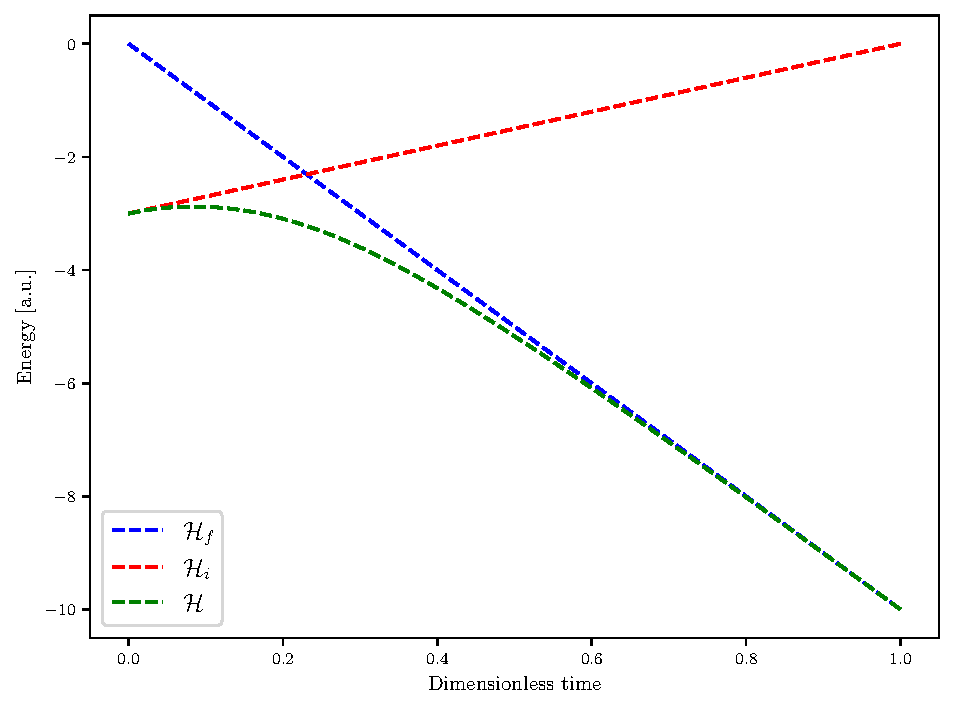
\includegraphics[width=\textwidth]{Figures/Two-Heirs.pdf}
    \caption{Eigenenergies of the ground state for the target, initial and total Hamiltonians. At $s=0$ the Hamiltonian of the system is dominated by $\mathcal{H}_{i}$, as $s$ increases the Hamiltonian is an interpolation of $\mathcal{H}_{i}$ and $\mathcal{H}_{f}$ and at $s=1$ the dominant Hamiltonian is $\mathcal{H}_{f}$ which is the one that encodes the solution to our problem.}
    \label{fig:HamiltonianInterpolation}
\end{figure}
This means that we get a global minimum value $E_{g}(s=1)$ associated with the ground states $\{\ket{\downarrow\uparrow\downarrow},\ket{\uparrow\downarrow\uparrow}\}$. This is because in this case, the problem has a degenerate ground state and the eigenvectors correspond to different configurations of our binary variables that lead to the same absolute minimum value $E_{g}(s=1)$. Intuitively, if a solution $\ket{\uparrow\downarrow\uparrow}$ indicates that Alice receives assets with indices $[0,2]$ and Bob receive the asset with index $[1]$, the opposite is a solution $\ket{\downarrow\uparrow\downarrow}$ with the same cost, i.e., Bob receives assets with indices $[0,2]$ and Alice receives the asset with index $[1]$.
%%%%%%%%%%%%%%%%%%%%%%%%%%%%%%%%%%%%%%%%%%%%%%%%%%%%%%%
\section{Circuit Based AQC: A First Approach}
In this section we sketch the idea of how to reproduce AQC in the gate model of computation with arbitrary precision. For a deeper understanding see Ref.\,\cite{Farhi2014AAlgorithm}.\\\\
According to Schrödinger equation, the evolution of a quantum system is given by
\begin{equation}
\ket{\psi(t)} = e^{-i\frac{\mathcal{H}}{\hbar}t} \ket{\psi(0)}.
\end{equation}
The previous equation represents a continuous evolution in time. This evolution can be simulated by a gate model circuit by discretizing the time evolution.\\\\
From the definition of the exponential of an operator $\hat{A}$
\begin{equation}
    e^{\hat{A}}=\lim_{n\rightarrow \infty}\left( 1 + \frac{\hat{A}}{n}\right)^{n},
\end{equation}
we can compute the exponential of a sum of operators as
\begin{equation}
    e^{\hat{A}+\hat{B}}=\lim_{n\rightarrow \infty}\left( 1 + \frac{\hat{A} + \hat{B}}{n}\right)^{n} = \lim_{n\rightarrow \infty}\left(e^{\hat{A}/n}e^{\hat{B}/n}\right)^{n}.
\end{equation}
According to the Suzuki-Trotter expansion of first order we can approximate the exponential of a sum of matrices by
\begin{equation}
        e^{\left(\hat{A}+\hat{B}\right)\Delta t} = e^{\hat{A}\Delta t}e^{\hat{B}\Delta t} + \mathcal{O}(\Delta t^{2}).
\end{equation}
In order to reproduce AQC with gates, we must discretize the time evolution in a set of time steps, $N$, of step size $\Delta t = T/N$,
\begin{align}
    e^{-i\hat{\mathcal{H}}\Delta t} = e^{-i\hat{\mathcal{H}}_{i}\beta(\Delta t)}e^{-i\hat{\mathcal{H}}_{f}\gamma(\Delta t)} + \mathcal{O}(\Delta t^{2}),
\end{align}
where
\begin{equation}
    e^{-i\hat{\mathcal{H}}_{i}\beta} = \prod_{k=1}^{N}e^{-i\left(T-k\Delta t\right)\hat{\mathcal{H}}_{i}}, \quad e^{-i\hat{\mathcal{H}}_{f}\gamma} = \prod_{k=1}^{N}e^{-i\left(k\Delta t\right)\hat{\mathcal{H}}_{f}}
\end{equation}
represents the time discretization of the initial and target Hamiltonians respectively. \\\\
Hence, we can decompose the adiabatic evolution operator $\hat{U}(T,0) = e^{-i\mathcal{H}(t)}$ in a product of exponentials
\begin{equation}
    \ket{\psi(t = T)} = \hat{U}(T,0)\ket{\psi(t = 0)} \simeq \prod_{k=1}^{N}e^{-i\left(T-k\Delta t\right)\hat{\mathcal{H}}_{i}}e^{-i\left(k\Delta t\right)\hat{\mathcal{H}}_{f}}\ket{\psi(t = 0)}. 
\end{equation}
In the limit $N \rightarrow \infty$ the gate model reproduces exactly the adiabatic evolution.
%%%%%%%%%%%%%%%%%%%%%%%%%%%%%%%%%%%%%%%%%%%%%%%%%%%%%%% 
%% Chapter 3

\chapter{Hybrid Methods} % Main chapter title

\label{Chapter3} % For referencing the chapter elsewhere, use \ref{Chapter2} 
%%%%%%%%%%%%%%%%%%%%%%%%%%%%%%%%%%%%%%%%%%%%%%%%%%%%%%%%%%%%%%%%%%%%%%%%%%%%%%%
% Hybrid classical-quantum annealing algorithm
%%%%%%%%%%%%%%%%%%%%%%%%%%%%%%%%%%%%%%%%%%%%%%%%%%%%%%%%%%%%%%%%%%%%%%%%%%%%%%%
Quantum computers are not mature enough to solve real-world problems. For instance, the embedding of a QUBO problem into the architecture of a quantum annealer impose a big constraint in the number of variables our problem can have. For this reason, a \textit{hybrid quantum-classical} (HQC) approach is currently the best method one can use to solve large-scale problems, by combining quantum and classical solvers.\\\\
The aim of hybrid quantum-classical approaches is to decompose a problem into a sub-problem(s) and master problem. Hopefully, one of these problems is a QUBO problem or can be cast into it, and it is small enough so it is assigned to the \textit{quantum processing unit} (QPU), meanwhile the other problems are solved by the classical solver using cutting-edge algorithms. \\\\
The problems we are interested have the following cost function,
\begin{equation}
    \mathcal{H} = \underbrace{\sum_{k=1}^{L}c_{k}^{(\text{iv})}l_{k}}_{\text{Investment Cost}} + \underbrace{\sum_{t=1}^{T}\sum_{j=1}^{G}c_{j}^{(\text{oc})}g_{j}(t)}_{\text{Operational Cost}}\\ 
\end{equation}
subject to a set of linear constraints,
\begin{align}
    0 \leq g_{j,t}\leq g_{j}^{\max},\quad \forall j,t \\
    D_{i}(t) =\sum_{j=1}^{G}g_{j}(t), \quad \forall i,t \\
\end{align}
Notice that the constraints are not binary either integer but real constraints. In order to represent a real constraint with a binary expansion one have to do a discretization process so that errors will appear due to that discretization. Hence, we should tackle the constraints with the classical solvers, otherwise many slack variables will be added to our QUBO problem and discretization errors will occur.
%%%%%%%%%%%%%%%%%%%%%%%%%%%%%%%%%%%%%%%%%%%%%%%%%%%%%%%%%%%%%%%%%%%%%%%%%%%%%%%
% QA + SA
%%%%%%%%%%%%%%%%%%%%%%%%%%%%%%%%%%%%%%%%%%%%%%%%%%%%%%%%%%%%%%%%%%%%%%%%%%%%%%%
\section{Hybrid classical-quantum annealing algorithm}
In Appx.\,\ref{AppendixB}, we show the foundations of \textit{simulated annealing} algorithm (SA) and solve a travelling salesman problem to illustrate it. A simulated annealing algorithm does not guarantee to get the optimal solution but the results we can get with a good annealing schedule are good enough in accuracy and time. Analogously with a quantum annealing algorithm. In this section, we illustrate the decomposition of a QUBO problem into two parts. A sub-problem solved by simulated annealing on a classical solver. A master problem addressed to a quantum annealer such that a embedding is possible.
%%%%%%%%%%%%%%%%%%%%%%%%%%%%%%%%%%%%%%%%%%%%%%%%%%%%%%%%%%%%%%%%%%%%%%%%%%%%%%%
\subsection{SA-QA protocol}
The hybrid quantum-classical algorithm based on combining SA with QA is inspired on\,\cite{Ding2019ImplementationDesign}. In that work, the authors proposed the following structure of the hybrid algorithm for a QUBO problem:
\begin{figure}[H]
\centering
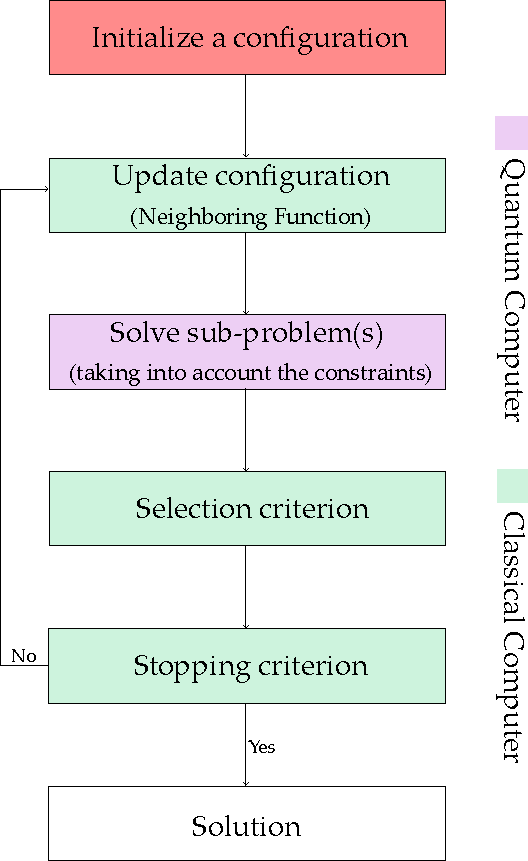
\includegraphics[width=0.5\textwidth]{Figures/SAQAProtocol_Layer 1.pdf} 
\caption{SA-QA protocol scheme.}
\label{fig:SA_QAProtocol}
\end{figure}
\begin{enumerate}
    \item Set the cost to a high value and initialize a configuration for the problem, i.e., annealing schedule, initial and final temperature, and a selection criterion.
    \item Randomly generate a new configuration by changing the values of the binary variables according to a neighboring function that generate a new configuration in one of this ways:
    \begin{enumerate}
        \item Randomly pick a binary variable with value 1 and set it to 0.
        \item Randomly pick a binary variable with value 0 and set it to 1.
        \item Randomly pick two binary variables with different values and swap them.
    \end{enumerate}
    \item Given the new configuration, solve the operational cost problem taking into account the constraints with a quantum annealing algorithm.
    \item Apply the selection criterion to keep or to discard the current configuration.
    \item Repeat steps 2 to 4 until a iteration index is equal to the upper value, then decrease the temperature and reset the iteration index.
    \item Outputs the current cost function value and its solution $\vec{x}$ when a stopping criterion is satisfied.
\end{enumerate}
Notice that the algorithm solve the master problem with a simulating annealing algorithm in a classical solver and then the sub-problem(s) -- which carries the constraints -- with the quantum computer, more precisely with a quantum annealer. For this reason, the sub-problem(s) must have binary constraints or integer if we do not want to deal with discretization errors. Hence, the approach as stated before is not for problems whose sub-problem(s) has real constraints meanwhile the master problem is more suitable for a quantum annealer.\\\\
In order to apply both simulated and quantum annealing to problems with real constraints, we have to reconsider or adapt the previous scheme.

%%%%%%%%%%%%%%%%%%%%%%%%%%%%%%%%%%%%%%%%%%%%%%%%%%%%%%%%%%%%%%%%%%%%%%%%%%%%%%%
% BD
%%%%%%%%%%%%%%%%%%%%%%%%%%%%%%%%%%%%%%%%%%%%%%%%%%%%%%%%%%%%%%%%%%%%%%%%%%%%%%%
\section{Benders' Decomposition}
The main idea behind Benders decomposition is that some problems simplify drastically if some variables are fixed, i.e., if some variables act as parameters. For this reason, the original problem is decompose into two problems with fixed variables. Firstly, a master problem with a subset $x^{m)}_{i} \subset \mathcal{W}$ of the original variables and its constraints is solved, then a sub-problem, which is the original problem with $x^{m)}_{i}$ fixed by the solution of the master problem, is solved. The solution of the master problem generates a lower bound, meanwhile the solution of the sub-problem generate an upper bound. Both problems are solved interactively according to some criteria until lower and upper bound are as close as the precision we want $\epsilon$.

%%%%%%%%%%%%%%%%%%%%%%%%%%%%%%%%%%%%%%%%%%%%%%%%%%%%%%%%%%%%%%%%%%%%%%%%%%%%%%%
% BD
%%%%%%%%%%%%%%%%%%%%%%%%%%%%%%%%%%%%%%%%%%%%%%%%%%%%%%%%%%%%%%%%%%%%%%%%%%%%%%%
\subsection{Classical Benders decomposition}
\textit{Classical Benders decomposition} (CBD) is a method to solve \textit{mixed integer programming} problems (MIP), but also MILP problems. These type of problems are combinatorial optimization problems, i.e., their goal is to find the combination of variables $x_{i}$ that minimises a given function, known as cost function subject to some integer constraints.\\\\
Suppose we are given a large optimization problem with many decision variables $\left(x_{0}^{m)}, x_{1}^{m)}, \hdots , x_{n}^{m)}, x_{0}^{s)}, x_{1}^{s)}\hdots x_{m}^{s)}\right)$ where the index $m$ indicates the variables associated with the master problem, and $s$ the variables associated with the sub-problem. The solution both problems find has to be consistent with the original problem, i.e., the constraints have to be fulfilled.\\\\
In the first iteration we have to fix the variables $x_{i}^{m)}$ to a feasible value and solve the sub-problem according to that fixed values. Once the sub-problem is solved
%%%%%%%%%%%%%%%%%%%%%%%%%%%%%%%%%%%%%%%%%%%%%%%%%%%%%%%%%%%%%%%%%%%%%%%%%%%%%%%
% BD: Multi-Cuts
%%%%%%%%%%%%%%%%%%%%%%%%%%%%%%%%%%%%%%%%%%%%%%%%%%%%%%%%%%%%%%%%%%%%%%%%%%%%%%%
\subsection{Hybrid Quantum-Classical Multi-cut Benders Approach}
In this section we present the protocol of a hybrid quantum-classical approach that has been applied to power system applications, see Ref.\,\cite{Paterakis2021HybridApplication}.\\\\


%----------------------------------------------------------------------------------------

% Define some commands to keep the formatting separated from the content 
\newcommand{\keyword}[1]{\textbf{#1}}
\newcommand{\tabhead}[1]{\textbf{#1}}
\newcommand{\code}[1]{\texttt{#1}}
\newcommand{\file}[1]{\texttt{\bfseries#1}}
\newcommand{\option}[1]{\texttt{\itshape#1}}

%----------------------------------------------------------------------------------------




%% Chapter 4
\chapter{Transmission Expansion Planning by Quantum Annealing} % Main chapter title
\label{Chapter4} % For referencing the chapter elsewhere, use \ref{Chapter1} 
\section{Statement of the Problem}
The \textit{Transmission expansion planning} (TEP)\,\cite{Neumann2020TransmissionFlows} problem determines the number of new lines to be installed in order to achieve a specific goal, optimizing the performance of an energy system subject to the assumptions of a future scenario. It is classically formulated as a \textit{mixed integer linear programming} (MILP) problem that aims at finding the optimal way to expand the capacity of an energy system by minimizing the cost function, which is the sum of the investment cost of transmission lines and the operational cost of generators. It decides how many transmission lines to build and where to connect them in order to satisfy the energy demand on a distributed energy system with a high share of renewable energy sources. There are other components to build apart from transmission lines such as generators or storages, but considering them implies not only an increment in the number of variables of the problem but also an increment in its complexity. For this reason, the problem we are solving is not completely realistic but it encapsulates the most important features of it. We should consider it just as a starting point to get insight about the problem formulation and challenges.\\\\
We can control the number of variables of the problem according to
\begin{itemize}
    \item \textbf{Number of nodes:} clustering techniques allow us to fix the number of nodes of the problem so that some loads of a given network are grouped acting as a single big load.
    \item \textbf{Snapshots of time}: in expansion problems it is common to consider hourly snapshots of time of one year, i.e., a total of 8760 snapshots. However, we can restrict the problem to a subset of snapshots without loss of generality.
    \item \textbf{Connectivity of transmission lines}: we can control the connectivity between nodes so that we do not allow a node the possibility of being fully connected with the rest of nodes. Furthermore, because of legal procedures to build new lines in areas where there are no transmission lines, TEP focuses on building lines in existing connections without changing the topology of the network.
    \item \textbf{Adding targets}: in this chapter we minimize the cost function as function of the investment cost of transmission lines, operational cost of generators and the load shedding cost, which is going to be explained later. But, there are other targets such as the increment of renewable energy sources in a given region or the reduction of the carbon footprint that we are not taking into account.
\end{itemize}
The resolution of MILP associated to TEP scales badly using classical algorithms\,\cite{Oertel2014ComplexityEvaluation} and, at the same time, energy system models are getting larger and more complex due to the integration of decentralized weather-dependent renewable energy sources, intermittent loads, sector coupling and the increase of storage components. Currently, the problem is often linearized or the scope and granularity of the model are reduced using clustering algorithms. For this reason, any computational time reduction will have substantial implications in closing the granularity gap between what the current models can solve and the desired resolution needed by energy system operators. However,  since quantum computers are still not sufficiently mature, large TEP problems cannot be solved fully by a quantum annealer. For this reason, we require hybrid methods\,\cite{Dilwali2016,Binato2001,Huang2019,MacRae2016,Zhao2021HybridProgrammingb} to decompose large problems into a master problem, which can be solved by a quantum annealer, and a sub-problem for which cutting-edge classical algorithms are going to be applied.
%%%%%%%%%%%%%%%%%%%%%%%%%%%%%%%%%%%%%%%%%%%
\subsection{Nomenclature}
In this section we introduce the notation of the TEP problem. Let $N$ be the set of nodes of a given network, $H$ the set of snapshots, $C$ the set of candidate transmission lines and $E$ the set of existing lines. Then $x_{kl}$, with $kl \in C$, represents the binary variable of the transmission line from node $k\in N$ to $l\in N$ -- it decides if that transmission line is built $x_{kl} = 1$ or not $x_{kl} = 0$ --, $d_{k}(h)$ represents the demand at node $k\in N$ in snapshot $h\in H$, $f_{kl}^{0}$  with $kl \in E$ represents the power flow being transmitted in existing line from node $k\in N$ to $l\in N$, $\bar{f}_{kl}^{0}$  with $kl \in E$ represents the maximum power flow being transmitted in existing line from node $k\in N$ to $l\in N$, $f_{kl}^{1}$  with $kl \in C$ represents the power flow being transmitted in candidate line from node $k\in N$ to $l\in N$, $\bar{f}_{kl}^{1}$  with $kl \in E$ represents the maximum power flow being transmitted in existing line from node $k\in N$ to $l\in N$, $g_{k}$ represents the energy produced at node $k\in N$, $\bar{g}_{k}$ represents the maximum energy production at node $k\in N$ and $r_{k}$ represents the load shedding, which can be thought as an artificial generator with a very large operational cost. Lastly, $c_{kl}$ is the coefficient of investment cost of transmission line from node $k \in N$ to $l \in N$, $c_{k}^{\text{oc}}$ is the operational cost of generator $k \in N$ and $c_{k}$ is the load shedding cost associated with $r_{k}$.
\begin{table}[H]
\centering
\begin{tabular}{|c|l|c|} 
 \hline	
 \textbf{Symbol} & \textbf{Description} & \textbf{Type} \\
 \hline	
 $N$ & Set of nodes of the network & Set\\
  \hline	
  $H$ & Set of snapshots & Set\\
  \hline
 $C$ & Set of candidate transmission lines & Set\\
    \hline	
 $C_{k}$ & Set of candidate transmission lines from all nodes to node $k$ & Set\\
  \hline	
 $E$ & Set of existing transmission lines & Set\\
   \hline	
 $E_{k}$ & Set of existing transmission lines from all nodes to node $k$ & Set\\
  \hline	
 $x_{kl}$ & Transmission line from node $k$ to $l$ & Binary\\
    \hline	
 $f_{kl}^{0}$ & Power flow in existing line from node $k$ to $l$ & Integer\\
     \hline	
 $\bar{f}_{kl}^{0}$ & Maximum power flow in existing line from node $k$ to $l$ & Integer\\
   \hline	
 $f_{kl}^{1}$ & Power flow in candidate line from node $k$ to $l$ & Integer\\
  \hline
 $\bar{f}_{kl}^{1}$ & Maximum power flow in candidate line from node $k$ to $l$ & Integer\\
 \hline
  $r_{k}$ & Shedding load at node $k$ & Integer\\
  \hline	
 $d_{k}(h)$ & Demand of node $k$ at snapshot $h$ & Integer\\
  \hline	
 $g_{k}(h)$ & Current generation at node $k$ at snapshot $h$ & Integer\\
  \hline	
 $\bar{g}_{k}$ & Maximum generation at node $k$ & Integer\\
   \hline
  $c_{kl}$ & Investment cost of transmission line from node $k$ to $l$ & Real\\
  \hline	
  $c_{k}^{(\text{oc})}$ & Annualised operational cost per MWh of generator $g_{k}$ & Real\\
  \hline
  $c_{k}$ & Cost of shedding load at node $k$ & Real\\
  \hline
\end{tabular}
\caption{Description of variables involved in TEP problems\,\cite{Dilwali2016}.}
\label{table:TEPNomenclature}
\end{table}
\subsection{Brownfield and Greenfield Models}
There are two ways of formulating the TEP, shown in Figure\,\ref{fig: ThreeNode}. On the one hand, the brownfield model considers the power flow of existing lines in a network $f_{kl}^{0}$ among with the power flow of a set of candidate lines $f_{kl}^{1}$. On the other hand, the greenfield model considers an empty network and a set of candidate lines $f_{kl}^{1}$. For simplicity, we are going to consider the greenfield approach so that we do not have to take into account the constants associated with the existing lines. We can map two indices $ij$ to a single index $k$ by using a bijective function for a given number of nodes $N$, see Ref.\,\cite{Jain2021SolvingComputer},
\begin{equation}
k(i,j,N) = \begin{cases}
    iN - i\left(i+1\right)/2 + j - (i+1)\ , & i<j\\
    \text{None}\ ,& i=j \\
    k(j,i,N)\ , & i>j
\end{cases}
    \label{eq: TwoIndexesmap}
\end{equation}
\begin{figure}[H]
  \begin{center}
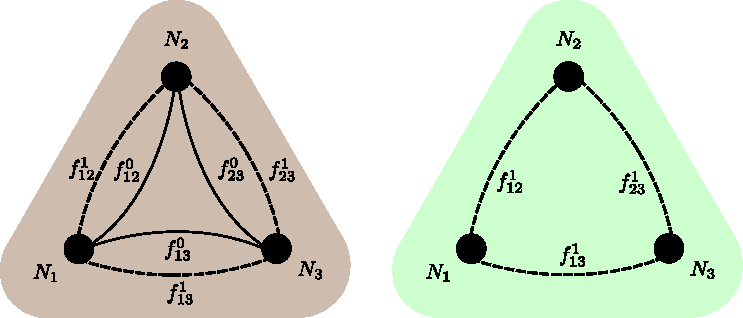
\includegraphics[width=0.8\textwidth]{Figures/3NodeBrownGreen.pdf}
  \end{center}
  \caption{Three node example. \textbf{Left:} Network considering current transmission lines -- solid lines -- and candidate lines -- dashed lines --, brownfield model. \textbf{Right:} Network considering just candidate lines, greenfield model.}
  \label{fig: ThreeNode}
\end{figure}
Luckily, the \textit{dimod} python package from D-Wave allows us to work with two indices so that we do not need to use the previous function to reformulate the problem. 
\subsection{Network Topology}
The TEP problems usually consider the building of new lines in existing connections so that we do not change the network topology. One of the reasons for adding lines in existing connections is because the legal permissions are granted. However, in a future scenario with a high share of decentralized renewable energies, new connections have to be considered. Hence, we are going to enable new connections by changing the topology. Moreover, we allow all lines to be connected to each node, i.e., we are considering fully connected networks.
\subsection{Formulation}
We formulate the TEP problem according to the work of Dilwali \textit{et al.}\,\cite{Dilwali2016} as follows
\begin{mini!}[2]
	{\mathbf{x},\mathbf{g},\mathbf{r},\mathbf{f}^{0},\mathbf{f}^{1}}{\underbrace{\sum_{kl\in C}c_{kl}x_{kl}}_{\textrm{Investment cost}} + \underbrace{\sum_{h\in H}\sum_{k}c_{k}^{(\textrm{oc})}g_{k}(h)}_{\textrm{Operational cost}} + \underbrace{\sum_{h\in H}\sum_{k}r_{k}(h)c_{k}}_{\textrm{Load shedding cost}} \label{eq: objective}}{\label{eq:StatementTEP}}{}
	\addConstraint{d_{k}(h)-\left(\sum_{l\in E_{k}}f_{kl}^{0}(h) + \sum_{l\in C_{k}}f_{kl}^{1}(h) + g_{k}(h) + r_{k}(h)\right)}{=0\ ,\quad}{\forall k\in N ,h\in H}{\label{const: PowerBalance}}
    \addConstraint{\abs{f_{kl}^{0}(h)} - \bar{f_{kl}^{0}}(h)}{\leq 0\ ,}{\forall\, kl \in E,h\in H }{\label{const: ExistingLimits}}
     \addConstraint{\abs{f_{kl}^{1}(h)} - \bar{f_{kl}^{1}}(h)x_{kl}}{\leq 0\ ,}{\forall\, kl \in C,h\in H }{\label{const: CandidateLimits}}
     \addConstraint{g_{k}(h)-\bar{g}_{k}(h)}{\leq 0\ ,}{\forall\, k\in N,h\in H }{\label{const: BusLimits}}
    \addConstraint{r_{k}(h) - d_{k}(h)}{\leq 0\ ,}{\forall\, k \in N,h\in H }{\label{const: BusLoads}}
    \addConstraint{\mathbf{d}, \mathbf{g}, \mathbf{f}^{0}, \mathbf{f}^{1}}{\geq 0}{}{}
    \addConstraint{x_{kl}}{\in \{0,1\}\ ,}{\forall\, kl \in C,}  
\end{mini!}
where the variables are described in Table\,\ref{table:TEPNomenclature}. We next briefly describe each equation:
\begin{itemize}
    \item \textbf{Objective function Eq.\,\eqref{eq: objective}}: it is the sum of investment cost of transmission lines, operational cost of generators and load shedding cost.
    \item \textbf{Power balance Eq.\,\eqref{const: PowerBalance}}: it represents the power balance constraints, i.e., if the demand $d_{k}(h)$ at node $k$ and snapshot $h$ is fulfilled by the generator $g_{k}$ at node $k$ and the power flow incoming from other nodes $f_{kl}^{0}(h)$ and $f_{kl}^{1}(h)$. The term $r_{k}$ is the load shedding. It can be thought of as an artificial generator whose operational cost is very large. It represents the fine for not fulfilling the demand in a node and it guarantees that the problem is feasible. To ensure that mathematically the demand is always fulfilled one can consider a load shedding term that is zero when demand at node $k$ is satisfied by the elements of the network and $r_{k} \neq 0$ when it is not fulfilled. If $r_{k} \neq 0$ the demand is not fulfilled, i.e., the electricity markets cannot offer the required energy to a given node and then pay a fine, which is an extra cost in the objective function. If the load shedding cost is high enough the demand is going to be always fulfilled since the load shedding term is the dominant term we want to minimize.
    \item \textbf{Existing circuit flow limits Eq.\,\eqref{const: ExistingLimits}}: the power flow of an existing transmission $f_{kl}^{0}$ line cannot exceed its maximum capacity, $\bar{f}_{kl}^{0}$.
    \item \textbf{Candidate circuit flow limits Eq.\,\eqref{const: CandidateLimits}}: the power flow of a candidate transmission line $f_{kl}^{1}$ cannot exceed its maximum capacity, $\bar{f}_{kl}^{1}$.
    \item \textbf{Node generation limits Eq.\,\eqref{const: BusLimits}}: the energy produced in a node $k$, $g_{k}$, cannot exceed its maximum energy production, $\bar{g}_{k}$.
    \item \textbf{Node loads limits Eq.\,\eqref{const: BusLoads}}: the load shedding at node $k$, $r_{k}$, cannot exceed the load $d_{k}$ of that node. 
\end{itemize}
\subsection{Remarks}
The previous model is called a transport model since we are not considering Kirchoff's equations. Notice that we include the operational cost which is usually not included in the literature\,\cite{Gomes2019}. The reason for usually not including the operational cost is that other authors consider a single snapshot so that the dominant term is the investment cost. However, if one wants to consider a large number of snapshots, then the operational cost is the dominant term. On the other hand, if we minimize the investment cost, then there is a change of building transmission lines that connect the most expensive generators to the nodes. In summary, extremal solutions lead to a high value of the cost function in one of the following ways:
\begin{itemize}
    \item \textbf{Underinvestment} leads to a high value of the total cost function because the system is not able to fulfill the demand $d(h)$.
    \item \textbf{Overinvestment} leads to a high value of the total cost function even though it satisfies the demand. Intuitively, we are creating more lines $\{x_{kl}\}$ than we need. Usually, there is an upper bound due to the capital budget.
\end{itemize}
The investment cost $c_{kl}$ is the cost of building the transmission line $x_{kl}$ and it is a constant -- we are not considering time-dependent costs. Analogously, the operational cost $c_{j}^{(\textrm{oc})}$ represents the annualised cost per MWh of the produced energy $g_{k}(h)$ at snapshot $h$. For simplicity, we set the operational cost to each carrier -- wind turbine, solar or run of river among others -- to a fixed value -- mean cost of that carrier -- so that we do not have to consider the variation of the cost as function of the node or the time.\\\\
Notice that when the solution is feasible, i.e., $r_k = 0$ for all $k\in N$, then the total cost depends on the investment cost and the operational cost. As stated before, the number of possible configurations of our problem scales badly. For this reason, knowing if we are considering a large set of snapshots -- large investment planning - or a small subset of snapshots gives us clues about what region of the configuration space we should explore. There are two regions to be considered:
\begin{itemize}
    \item \textbf{Large expansion planning:} for instance if we consider a 10 year expansion planning problem and we produce the energy with the cheapest carriers -- e.g. wind turbines -- we will reduce the operational cost drastically as compared with producing the energy with other carriers. However, it is possible that the fact of producing the energy with the cheapest carriers implies the need of building the most expensive transmission lines, hence increasing the investment cost.
    \item \textbf{Short expansion planning:} for instance if we consider a single-snapshot.  Then, it is clear that the minimum total cost function implies a minimum in the investment cost regardless of the operational costs, since the operational costs are lower as compared with the investment cost when there is only one snapshot to optimize over.
\end{itemize}
To summarise, given the energy demand for a set of nodes $N$ for a set of snapshots $H$, the goal is to optimise the network so as to build the minimum amount of transmission lines -- minimizing in that way the investment cost -- while satisfying the energy demand for each snapshot. We are also taking into account the operational cost of each carrier so there is a trade-off between the investment cost of transmission lines and the operational cost of generators used to produce the energy to satisfy the demand.
%%%%%%%%%%%%%%%%%%%%%%%%%%%%%%%%%%%%%%%%%%%%%%%%%%%%%%%%%%%%%%%%%%%%%%%%%%%%%%%%%%
%       SOLVING A SMALL PROBLEM WITH A REAL QUANTUM ANNEALER
%%%%%%%%%%%%%%%%%%%%%%%%%%%%%%%%%%%%%%%%%%%%%%%%%%%%%%%%%%%%%%%%%%%%%%%%%%%%%%%%%%
\newpage
\section{Small Network solved by D-Wave's simulators}
 We are considering a single snapshot of a three-node fully-connected network with nonexistent lines with a single demand at node $2$ and without the load shedding term. Furthermore, each node has a single generator $g_{k}$ with a nominal power -- maximum capacity -- of $10$ energy units.
 \begin{table}[H]
\centering
\begin{tabular}{ |c |c| c| }
  \hline			
  \textbf{Symbol} & \textbf{Description} & \textbf{Value}  \\
    \hline		
   $\mathbf{c} = \left[c_{12},c_{13},c_{23}\right]$ & Investment cost & $\left[10, 20, 30\right]$\\
       \hline		
   $\mathbf{c}^{\textrm{oc}} = \left[c_{1}^{\textrm{oc}},c_{2}^{\textrm{oc}}, c_{3}^{\textrm{oc}}\right]$ & Operational cost & $\left[10, 5, 2\right]$\\
          \hline		
   $\mathbf{d} = \left[d_{1}, d_{2}, d_{3}\right]$ & Demands & $\left[0, 12, 0\right]$\\
       \hline		
   $\mathbf{\bar{g}} = \left[\bar{g}_{1},\bar{g}_{2},\bar{g}_{3}\right]$ & Maximum capacity & $\left[10, 10, 10\right]$\\
    \hline	
    $\mathbf{\bar{f}}^{1} = \left[f_{12}^{1},f_{13}^{1},f_{23}^{1}\right]$ & Maximum Power Flow in candidate line & $\left[10, 10, 10\right]$\\
    \hline
\end{tabular}
\caption{Investment cost, operational cost, demand, maximum capacity per generator and maximum power flow per candidate line for a three node network.}
\label{tab:SmallNetwork}
\end{table}
We use synthetic data for our TEP problem described in Table\,\ref{tab:SmallNetwork}.\\
The objective function for the three node fully connected network described above is
\begin{mini!}[2]
	{\mathbf{x}, \mathbf{g}}{\underbrace{\mathbf{C}^{\intercal}\mathbf{x}}_{\textrm{Investment Cost}} + \underbrace{\mathbf{C}_{\textrm{oc}}^{\intercal}\mathbf{g}}_{\textrm{Operational Cost}}}{}{}{}
 	\addConstraint{g_{k}}{\leq \bar{g}_{k} }{\forall\, k \in N}{}
	\addConstraint{d_{k}}{= g_{k}  + \underbrace{\sum_{l\neq k, l\in N}g_{k}x_{kl}}_{\textrm{Quadratic Constraint}}}{\forall\, k \in N}{}
    \addConstraint{\mathbf{d}, \mathbf{g}}{\geq 0\,}{}{}
    \addConstraint{x_{kl}}{\in \{0,1\},\,}{\forall\, kl \in C}.
    \end{mini!}
Notice that we are not considering the power flow limits $f_{kl}^{1}$ of candidate lines. Any candidate line can transmit any amount of energy. In other words, we wrote the problem in such a way that none of the power flow limits is going to be violated, see Figure\,\ref{fig: Green_inital}.
\begin{figure}[H]
  \begin{center}
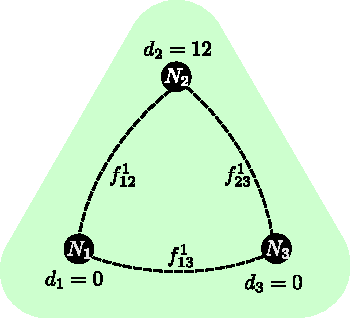
\includegraphics[width=0.4\textwidth]{Figures/Green_Initial.pdf}
  \end{center}
  \caption{Graphic formulation of three node problem.}
  \label{fig: Green_inital}
\end{figure}
The demand at node $2$ is $12$ energy units, so it cannot be fulfilled by its own generator and requires energy from at least one of the neighboring nodes which means we need to build at least one transmission line connected to node $2$.
\subsection{D-Wave CQM ExactSolver()}
Since the problem we are tackling has just a few variables we can sample all the configuration space. For this task we use the \textit{CQM ExactSolver} class. One of the advantage of CQM is that it writes down if the solution is feasible, i.e.,  if that solution satisfy all the constraints of our problem. The solution of the problem is represented graphically in Figure\,\ref{fig: Green_final}.
\begin{figure}[H]
  \begin{center}
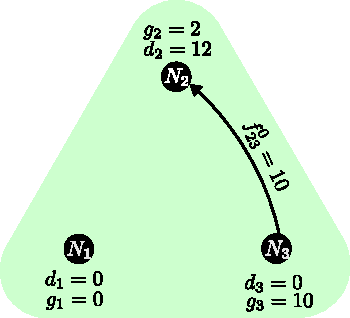
\includegraphics[width=0.4\textwidth]{Figures/Green_Final.pdf}
  \end{center}
  \caption{Graphical solution of three node problem.}
  \label{fig: Green_final}
\end{figure}
The Table\,\ref{tab:SmallNetworkResults} represents only feasible solutions which are sorted from lower energy to higher energy. The first row is the solution that minimizes the objective function by fulfilling the constraints, i.e., the demand.
 \begin{table}[H]
\centering
\begin{tabular}{ |c|c|c|c|c|c|c|c| }
  \hline			
  $\mathbf{x_{12}}$ & $\mathbf{x_{13}}$ & $\mathbf{x_{23}}$ & $\mathbf{g_{1}}$ & $\mathbf{g_{2}}$ & $\mathbf{g_{3}}$ & \textbf{Prices} & \textbf{Feasible} \\
  \hline
    0 & 0 & 1 & 0 & 2 & 10 & 60 & True \\
  \hline
    0 & 0 & 1 & 0 & 3 & 9 & 63 & True \\
  \hline
    0 & 0 & 1 & 0 & 4 & 8 & 66 & True \\
  \hline
    0 & 0 & 1 & 0 & 6 & 7 & 69 & True \\
  \hline
\end{tabular}
\caption{D-Wave's feasible solutions to the TEP combinatorial optimization problem.}
\label{tab:SmallNetworkResults}
\end{table}
The optimal solution decides to build the most expensive transmission line, i.e., the one connecting nodes 2 and 3, and to use the maximum capacity of the cheapest generator, the one at node 3, see Table\,\ref{tab:SmallNetwork}.
\subsection{D-Wave LeapHybridCQMSampler()}
The complete implementation of TEP problems -- taking into account integer or real variables -- requires of hybrid solvers. For this reason, we implemented the TEP problem from\,\eqref{eq:StatementTEP} in Python and use a D-Wave hybrid solver. As you may guess the results should be the same as the ones stated in the previous sections. However, in Table\,\ref{tab:SmallNetworkResultsHybrid} there are columns that did not appear before. The problem as stated here is general and takes into account every variable of TEP problems which do not happen with the formulation of last section.
 \begin{table}[H]
\centering
\begin{tabular}{ |c|c|c|c|c|c|c|c|c|c|c|c|c|c|c|c|c| }
  \hline			
  $\mathbf{x_{12}}$ & $\mathbf{x_{13}}$ & $\mathbf{x_{23}}$ & $\mathbf{f_{12}}$ & $\mathbf{f_{13}}$ & $\mathbf{f_{21}}$ & $\mathbf{f_{23}}$ & $\mathbf{f_{31}}$ & $\mathbf{f_{32}}$ &$\mathbf{g_{1}}$ & $\mathbf{g_{2}}$ & $\mathbf{g_{3}}$ & $\mathbf{r_{1}}$ & $\mathbf{r_{2}}$ & $\mathbf{r_{3}}$ &  \textbf{Prices} \\
  \hline
    0 & 0 & 1 & 0 & 0 & 0 & 10 & 0 & 0 & 0 & 2 & 10 & 0 & 0 & 0 & 60 \\
  \hline
  1 & 1 & 0 & 0 & 10 & 10 & 0 & 0 & 0 & 0 & 2 & 10 & 0 & 0 & 0 & 60 \\
  \hline
\end{tabular}
\caption{D-Wave's feasible solutions to the TEP combinatorial optimization problem.}
\label{tab:SmallNetworkResultsHybrid}
\end{table}
Notice that there are two solutions with the same cost. The first one has been shown in the previous section. However, the new solution produced by the hybrid solver build two lines whose accumulated cost is the same as the one connecting the node $3$ and the node $2$. Taking into account the complete formulation of the problem and not just a simplification allow us to get new solutions that otherwise do not appear. In this case, the complete formulation of the problem allow the current to flow between nodes until it reach the destination node.
\begin{figure}[H]
  \begin{center}
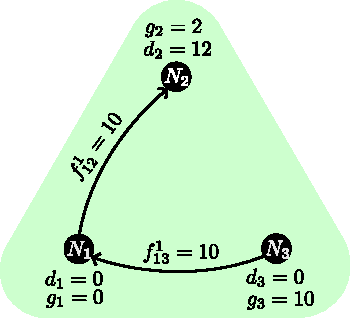
\includegraphics[width=0.4\textwidth]{Figures/3NodeGreenHybrid.pdf}
  \end{center}
  \caption{Graphical solution of three node problem.}
  \label{fig: Green_final_Hybrid}
\end{figure}
\subsubsection{Execution Times}
Last, we run ten test for a different number of nodes in a network with a D-Wave hybrid solver known as \textit{LeapHybridCQMSampler}. Despite the execution time of the hybrid solvers can be set, the LeapHybridSampler will calculate a minimum time based on the size of our problem. We let the hybrid sampler to decide the amount of time each problem requires. The execution times for a set of TEP problem is shown in Figure\,\ref{fig: ExecutionTimes}. 
\begin{figure}[H]
  \begin{center}
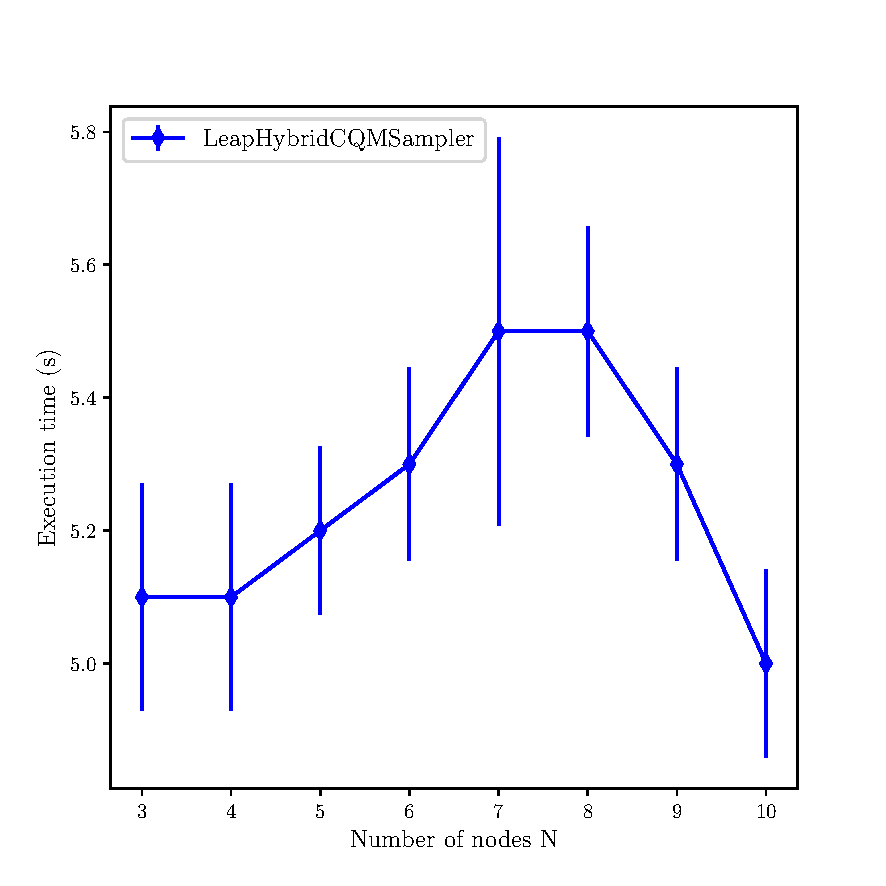
\includegraphics[width=0.8\textwidth]{Figures/ExecutionTimes.pdf}
  \end{center}
  \caption{Execution times for different test cases of small networks with D-Wave \textit{LeapHybridCQMSampler}.}
  \label{fig: ExecutionTimes}
\end{figure}
%%%%%%%%%%%%%%%%%%%%%%%%%%%%%%%%%%%%%%%%%%%%%%%%%%%%%%%%%%%%%%%%%%%%%%%%%%%%%%%%%%
%       BENDERS DECOMPOSITION for TEP [Large Problems]
%%%%%%%%%%%%%%%%%%%%%%%%%%%%%%%%%%%%%%%%%%%%%%%%%%%%%%%%%%%%%%%%%%%%%%%%%%%%%%%%%%
\section{Benders Decomposition in TEP}
In Chapter\,\ref{Chapter3} we showed three hybrid approaches that combine classical and quantum solvers. In this work, we decided to explore the Benders' decomposition approach due to two main points. Firstly, the convergence properties of Benders' decomposition allows us to know how good a solution is. Secondly, TEP problems have diagonal structure which means they are suitable for a Benders' decomposition approach. We propose a quantum Benders' decomposition scheme for a general formulation of TEP problems, but its implementation is left for a future work. However, the results of Figure\,\ref{fig: ExecutionTimes} will be be compared in the future with the results we get from our quantum BD algorithm.\\\\\
In order to simplify the problem we consider a single snapshot so that we can drop the $h$ index. As discussed in Ch.\,\ref{Chapter3}, we can formulate the problem by maximizing a dual function or by minimizing the primal problem with the dual as penalties. The Benders' decomposition algorithm that we propose consists of four steps:
\begin{itemize}
    \item \textbf{Step 1} (\textit{Initialization of Benders’ decomposition})\textbf{:} we initialize the iteration counter $t$, the upper bound $\bar{z}^{0}$, the lower bound $\underline{z}^{0}$, the load shedding and operational cost $\alpha^{0}$ and the penalty term associated with the violation of power flow constraints of candidate lines $\Pi_{f_{kl}^{1}}$.
    \item \textbf{Step 2} (\textit{Master problem solved by a quantum annealer})\textbf{:} we increase the lower bound $\underline{z}^{t}$ by taking the minimum value of 
        \begin{mini!}[2]
	   {\mathbf{x}}{\underline{z}^{t}}{}{}{}
	   \addConstraint{\underline{z}^{t} \geq \sum_{kl\in C}c_{kl}x_{kl}^{t} + \alpha^{t-1} - \underbrace{\sum_{kl\in C}\Pi^{\tau}_{f_{kl}^{1}}\left(x_{kl}^{t} - x_{kl}^{\tau}\right)}_{\textrm{Benders' cuts}}}{=0,}{\quad \forall \tau = 1,\hdots,t-1.}{}
        \end{mini!}
    In that equation $\alpha^{t-1}$ represent the summation of the objective function of the slave problem(s) and $\Pi_{f_{kl}^{1}}^{\tau}$ represent the Benders' cut of iteration $\tau$ where $\tau < t$, for the linking constraint of Eq.\,\eqref{const: CandidateLimits}. Notice that we have a Benders' cut for every candidate circuit flow constraint $f_{kl}^{1}$. In every iteration of Benders' algorithm we are adding cuts, in other words we are restricting the region of feasible solutions.
    \item \textbf{Step 3} (\textit{Slave problem solved by a classical solver})\textbf{:} we minimize $\alpha^{t}$ which includes the load shedding cost and the operational cost.
    \begin{mini!}[2]
	{\mathbf{g},\mathbf{r}, \mathbf{f}^{0}, \mathbf{f}^{1}}{\alpha^{t} \equiv \underbrace{\sum_{k}c_{k}^{(\textrm{oc})}g_{k}}_{\textrm{Operational cost}} + \underbrace{\sum_{k}r_{k}c_{k}}_{\textrm{Load shedding cost}}}{}{}{}
	\addConstraint{d_{k}-\left(\sum_{l\in E_{k}}f_{kl}^{0} + \sum_{l\in C_{k}}f_{kl}^{1} + g_{k} + r_{k}\right)}{=0,\quad}{\forall k\in N }{}
    \addConstraint{\abs{f_{kl}^{0}} - \bar{f}_{kl}^{0}}{\leq 0,\,}{\forall\, kl \in E}{}
     \addConstraint{\abs{f_{kl}^{1}} - \bar{f}_{kl}^{1}x^{t}_{kl}}{\leq 0,\,}{\forall\, kl \in C}{}
     \addConstraint{g_{k}-\bar{g}_{k}}{\leq 0,\,}{\forall\, k\in N}{}
    \addConstraint{r_{k} - d_{k}}{\leq 0,\,}{\forall\, k \in N}{}
    \addConstraint{\mathbf{d}, \mathbf{g}, \mathbf{f}^{0}, \mathbf{f}^{1}}{\geq 0\,}{}{\label{const: positivevalues}}.
    \end{mini!}
    \item \textbf{Step 4} (\textit{Stopping criterion})\textbf{:} after minimizing $\alpha^{t}$ we reduce the upper bound
    \begin{equation}
        \bar{z}^{t} = \min \{\bar{z}^{t-1}, \sum_{kl \in C}c_{kl}x_{kl}^{t} + \alpha^{t}\}.
    \end{equation}
    If the difference between the upper and lower bound is less or equal than a given threshold
    \begin{equation}
        \bar{z} - \underline{z} \leq \epsilon,
    \end{equation}
    then the Benders' algorithm stops and outputs the value of $\{\mathbf{x},\mathbf{g},\mathbf{r},\mathbf{f^{1}}\}$ as the (sub-)optimal solution. Otherwise, it goes to step 2 with the new candidate solution as input.
\end{itemize}

 
%% Chapter 5

\chapter{Results and discussion} % Main chapter title
\label{Chapter5} % For referencing the chapter elsewhere, use \ref{Chapter5} 
\section{Small Network solved by D-Wave CQM Sampler}
\subsection{D-Wave CQM ExactSolver()}
Since the problem we are tackling has just a few variables we can sample all the configuration space. For this task we use the \textit{CQM ExactSolver} class. One of the advantage of CQM is that it writes down if the solution is feasible, i.e.,  if that solution satisfy all the constraints of our problem. The solution of the problem is represented graphically in Figure\,\ref{fig: Green_final}.
\begin{figure}[H]
  \begin{center}
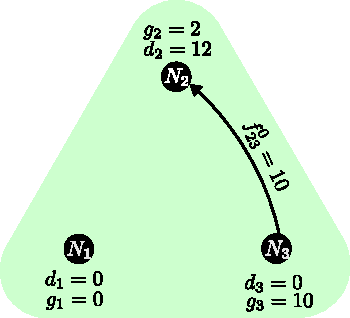
\includegraphics[width=0.4\textwidth]{Figures/Green_Final.pdf}
  \end{center}
  \caption{Graphical solution of three node problem.}
  \label{fig: Green_final}
\end{figure}
Notice that Table\,\ref{tab:SmallNetworkResults} represents only feasible solutions. They are sorted from lower energy to higher energy which means that the first row is the solution that minimizes the objective function by fulfilling the constraints, in this example the demand.
 \begin{table}[H]
\centering
\begin{tabular}{ |c|c|c|c|c|c|c|c| }
  \hline			
  $\mathbf{x_{12}}$ & $\mathbf{x_{13}}$ & $\mathbf{x_{23}}$ & $\mathbf{g_{1}}$ & $\mathbf{g_{2}}$ & $\mathbf{g_{3}}$ & \textbf{Prices} & \textbf{Feasible} \\
  \hline
    0 & 0 & 1 & 0 & 2 & 10 & 60 & True \\
  \hline
    0 & 0 & 1 & 0 & 3 & 9 & 63 & True \\
  \hline
    0 & 0 & 1 & 0 & 4 & 8 & 66 & True \\
  \hline
    0 & 0 & 1 & 0 & 6 & 7 & 69 & True \\
  \hline
\end{tabular}
\caption{D-Wave's feasible solutions to the TEP combinatorial optimization problem.}
\label{tab:SmallNetworkResults}
\end{table}
The optimal solution decides to build the most expensive transmission line, i.e., the one connecting nodes 2 and 3, and to use the maximum capacity of the cheapest generator, the one at node 3, see Table\,\ref{tab:SmallNetwork}.
%%%%%%%%%%%%%%%%%%%%%%%%%%%%%%%%%%%%%%%%%%%%%%%
\subsection{D-Wave LeapHybridCQMSampler()}
The implementation of TEP problems into D-Wave annealer requires of hybrid solvers due to the integers and real variables involved in the problem. For this reason, we implemented the  TEP problem from \textbf{INSERTAR RANGO DE ECUACIONES} in Python and use the D-Wave hybrid solver. As you may guess the results should be the same as the ones stated in the previous sections. However, in Table\,\ref{tab:SmallNetworkResultsHybrid} there are columns that did not appear before. The problem as stated here is general and takes into account every variable of TEP problems which do not happen with the formulation of last section.
 \begin{table}[H]
\centering
\begin{tabular}{ |c|c|c|c|c|c|c|c|c|c|c|c|c|c|c|c|c| }
  \hline			
  $\mathbf{x_{12}}$ & $\mathbf{x_{13}}$ & $\mathbf{x_{23}}$ & $\mathbf{f_{12}}$ & $\mathbf{f_{13}}$ & $\mathbf{f_{21}}$ & $\mathbf{f_{23}}$ & $\mathbf{f_{31}}$ & $\mathbf{f_{32}}$ &$\mathbf{g_{1}}$ & $\mathbf{g_{2}}$ & $\mathbf{g_{3}}$ & $\mathbf{r_{1}}$ & $\mathbf{r_{2}}$ & $\mathbf{r_{3}}$ &  \textbf{Prices} \\
  \hline
    0 & 0 & 1 & 0 & 0 & 0 & 10 & 0 & 0 & 0 & 2 & 10 & 0 & 0 & 0 & 60 \\
  \hline
  1 & 1 & 0 & 0 & 10 & 10 & 0 & 0 & 0 & 0 & 2 & 10 & 0 & 0 & 0 & 60 \\
  \hline
\end{tabular}
\caption{D-Wave's feasible solutions to the TEP combinatorial optimization problem.}
\label{tab:SmallNetworkResultsHybrid}
\end{table}
Notice that there are two solutions with the same cost. The first one has been shown in the previous section. However, the new solution produced by the hybrid solver build two lines whose cummalated cost is the same as the one connecting the node $3$ and the node $2$.
\begin{figure}[H]
  \begin{center}
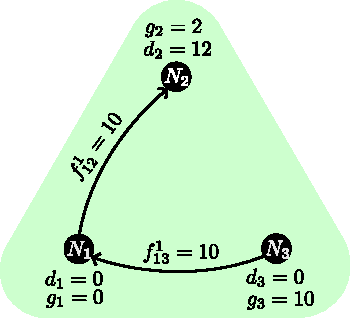
\includegraphics[width=0.4\textwidth]{Figures/3NodeGreenHybrid.pdf}
  \end{center}
  \caption{Graphical solution of three node problem.}
  \label{fig: Green_final_Hybrid}
\end{figure}
 

%----------------------------------------------------------------------------------------
%	THESIS CONTENT - APPENDICES
%----------------------------------------------------------------------------------------

\appendix % Cue to tell LaTeX that the following "chapters" are Appendices

% Include the appendices of the thesis as separate files from the Appendices folder
% Uncomment the lines as you write the Appendices

% Appendix A

\chapter{Introduction to Quantum Computing} % Main appendix title
This appendix serves as a quick introduction to quantum computing. We explain the basics concepts without going deeply into their physical meaning or historical approach. For a deeper discussion of the topics described herein, we refer the reader to Refs. \cite{W.Bryon1992HilbertFunctions},  \cite{Scherer2019MathematicsComputing} and \cite{Nielsen2010QuantumInformation}.
\label{AppendixA} % For referencing this appendix elsewhere, use \ref{AppendixA}
%%%%%%%%%%%%%%%%%%%%%%%%%%%%%%%%%%%%%%%%%%%%%%%%%%%%%%%%%%%%%%%%%%%%%%%%%%%%%%%%%%%%%%%%%%%%%%%%%%%%%%%%%%
%     A.1 HILBERT SPACE
%%%%%%%%%%%%%%%%%%%%%%%%%%%%%%%%%%%%%%%%%%%%%%%%%%%%%%%%%%%%%%%%%%%%%%%%%%%%%%%%%%%%%%%%%%%%%%%%%%%%%%%%%%
\section{Hilbert space}
We start by defining the vector space where quantum computing takes place, the Hilbert space, $\mathbb{H}$.
\begin{definition}[Hilbert Space]
A Hilbert space is a special type of linear vector space whose elements are complex-valued \textit{square integrable}\footnote{A function $\psi(x)$ is said to be \textit{square integrable} on a given interval $\left[a, b\right]$ if $\int_{a}^{b}\|\psi(x)\|^{2}dx$ exist with a finite value.} functions, $\psi(x)$, of a real variable $x$, defined on the closed interval $\left[a, b\right]$, equipped with a \textit{complete inner product}, $(\cdot,\cdot)$, in $\mathbb{C}$.
\end{definition}
\begin{definition}[Inner Product]
Given two functions of the Hilbert space, $\psi_{1}$ and $\psi_{2}$, the inner product is defined by
\begin{equation}
    \left(\psi_{1}, \psi_{2}\right) \equiv \int^{b}_{a} \psi_{1}^{*}(x)\psi_{2}(x)dx
\end{equation}
\end{definition}
\begin{corollary}
Given the functions \{$\psi_{1}$,$\psi_{2}$,$\psi_{3}$\} $\in \mathbb{H}$ and \{$\alpha, \beta\} \in \mathbb{C}$, the inner product of the associated Hilbert space satisfies:
\begin{itemize}
    \item Closed operation: $(\psi_{1},\psi_{2})\in \mathbb{C}$
    \item Conjugate symmetry: $(\psi_{1},\psi_{2}) = (\psi_{2},\psi_{1})^{*}$
    \item Linear with respect to the second vector: $(\psi_{1},\lambda \cdot \psi_{2} + \beta\cdot\psi_{3}) = \lambda(\psi_{1},\psi_{2}) + \beta(\psi_{1},\psi_{3})$
    \item Anti-linear with respect to the first vector: $(\lambda \cdot \psi_{1} + \beta \cdot \psi_{2}, \psi_{3}) = \lambda^{*}(\psi_{1},\psi_{3}) + \beta^{*} (\psi_{2},\psi_{3})$
    \item Positive definiteness: $(\psi, \psi) = \lVert \psi \rVert^{2} \in \left[0,\infty\right)$\footnote{The quantity $\lVert \psi \rVert^{2}$ is called the norm of $\psi$. If $\lVert \psi \rVert^{2} = 0$ that does not imply $\psi(x) = 0$ for all $x$ in $\left[a,b\right]$. The function can have nonzero values at some points and the integral will remain zero. The integral roughly computes the area in a given interval, so, if there is just a point not null in the interval the area captured by a point is zero, so its contributions to the integral is zero. In our case the quantity $\lVert \psi \rVert^{2}$ represents the probability density of a given state $\psi$, i.e., if we integrate the whole interval of definition $x \in D$, $\int_{D}\lVert \psi \rVert^{2}dx = 1$.} 
\end{itemize}    
\end{corollary}
\begin{definition}[Distance]
    The distance defined by Hilbert space's inner product is given by
    \begin{equation}
      d \equiv \left|\psi_{2} - \psi_{1}\right| = \sqrt{(\psi_{2}-\psi_{1},\psi_{2}-\psi_{1})}  
    \end{equation}
\end{definition}
\begin{definition}[Completeness of a space]
A complete space is one in which any Cauchy sequence -- of that space -- is convergent, i.e., tends towards a value inside the given space.
\end{definition}
We can show why completeness of space is a necessary condition. Suppose that our space is not complete, i.e., some Cauchy sequences are not convergent. Then, the evolution of an initial state\footnote{The formulae for the evolution of n state is explained in later sections.}, $\ket{\psi(0)}$, under a given constant Hamiltonian is not guaranteed\footnote{It is not guaranteed that the Cauchy sequence $\sum_{i = 0}^{n}(-it)^{k} / \left(k!h^{k}\right)\mathcal{H}^{k}$ converges.}
\begin{equation}
    \ket{\psi(t)} = e^{-\frac{i\mathcal{H}}{\hbar}t}\ket{\psi(0)} = \lim_{n \to \infty} \sum_{i = 0}^{n}\frac{(-it)^{k}}{k!h^{k}}\mathcal{H}^{k}\ket{\psi(0)}
\end{equation}
\begin{definition}[Completeness of an orthonormal set of functions]
A set of orthonormal functions $\{\psi_{i}\}$ is complete if any function $\psi(x)$ in Hilbert space can be written as a linear combination of the $\psi_{i}(x)$\footnote{Here we do not ask for point convergence, we weaken the converge criteria to mean convergence. Otherwise, there would not exist a complete set of orthonormal function in the Hilbert space.}:
\begin{equation}
    \lim_{n\to \infty}\| \psi(x) - \sum_{i=1}^{n}c_{i}\psi_{i}(x)\|^{2} = 0
\end{equation}
\end{definition}
\begin{theorem}[Riesz-Fischer]
Assume the functions $\psi_{1}(x),\psi_{2}(x),\ldots$ are elements of Hilbert space. If
\begin{equation}
    \lim_{n,m\to\infty} \lVert \psi_{n} - \psi_{m}\rVert^{2} \equiv \lim_{n,m\to \infty} \int_{a}^{b} \|\psi_{n} - \psi_{m}\|^{2}dx = 0
\end{equation}
then there exist a square (Lebesgue) integrable function $\psi(x)$ to which the sequence $\psi_{n}(x)$ converges such that 
\begin{equation}
    \lim_{n\to \infty} \int_{a}^{b} \|\psi - \psi_{n}\|^{2}dx = 0
\end{equation}
Equivalently, let $\psi_{n}$ be a Cauchy sequence and $\psi$ a value inside the given space. Then, the Cauchy sequence converges to $\psi(x)$ \textit{in the mean}, i.e, we allow the difference $\|\psi(x) - \psi_{n}(x)\|^{2}\neq 0$ at some points $x$, so that the integral $\lim_{n\to \infty} \int_{a}^{b} \|\psi - \psi_{n}\|^{2}dx$ is zero when taking into account the whole interval.
\end{theorem}
\begin{definition}[Orthonormality]
A given set of functions $\{\psi_{i}\}$ is said to be orthonormal if
\begin{equation}
    \left(\psi_{i}, \psi_{j}\right) \equiv \int_{a}^{b} \psi_{i}^{*}(x)\psi_{j}(x) dx = \delta_{ij} 
\end{equation}
\end{definition}
In the present work we work with a particular Hilbert space, a finite Hilbert space. This implies our space is \textit{separable}.
\begin{definition}[Separable]
    A Hilbert space is said to be \textit{separable} if an only if it has a countable orthonormal basis.
\end{definition}
So for a finite Hilbert space -- which is a countable space -- an orthogonal basis is guaranteed.
%%%%%%%%%%%%%%%%%%%%%%%%%%%%%%%%%%%%%%%%%%%%%%%%%%%%%%%%%%%%%%%%%%%%%%%%%%%%%%%%%%%%%%%%%%%%%%%%%%%%%%%%%%
%     A.2 NOTACION
%%%%%%%%%%%%%%%%%%%%%%%%%%%%%%%%%%%%%%%%%%%%%%%%%%%%%%%%%%%%%%%%%%%%%%%%%%%%%%%%%%%%%%%%%%%%%%%%%%%%%%%%%%
\section{Notation}
\begin{definition}[Dirac's Bra-Ket Notation]
The inner product of an n-dimensional Hilbert space defines a linear map from $\mathbb{H}$ to $\mathbb{C}$
\begin{align*}
  \tau: \mathbb{H}\longrightarrow& \mathbb{C}^{n} \\
  \tau(\psi) \longrightarrow& \begin{bmatrix}
           \alpha_{1} \\
           \vdots \\
           \alpha_{n}
         \end{bmatrix}
\end{align*}  
Conversely, 
\begin{align*}
  \bar{\tau}: \mathbb{H}^{*}\longrightarrow& \mathbb{C}^{n} \\
  \bar{\tau}(\psi)\longrightarrow& 
         \begin{bmatrix}
           \alpha_{1}^{*}, \hdots, \alpha_{n}^{*}
         \end{bmatrix}
\end{align*} 
where $\mathbb{H}^{*}$ denotes the dual space. The dual space $\mathbb{H}^{*}$ is also a Hilbert space with the same dimension as $\mathbb{H}$. 
\begin{itemize}
    \item Elements of a Hilbert space, $\mathbb{H}$ are called \textit{ket-vectors} 
\begin{equation}
    \psi \equiv \ket{\psi} =  \begin{bmatrix}
           \alpha_{1} \\
           \vdots \\
           \alpha_{n}
         \end{bmatrix}
\end{equation}
\item Elements of a dual Hilbert space $\mathbb{H}^{*}$ are called \textit{bra-vectors}
\begin{equation}
    \psi^{*} \equiv \bra{\psi} =  \begin{bmatrix}
           \alpha_{1}^{*}, & \hdots &, \alpha_{n}^{*}
         \end{bmatrix}
\end{equation}
\end{itemize}
\end{definition}

Notice that a bra-vector is just the transpose conjugate of a ket-vector. This is a useful way of mapping a ket-vector of a given Hilbert space into its bra-vector on the associated dual Hilbert space.

\begin{corollary}
    In bra-ket notation, a set of vectors $\{\ket{\psi_{j}}\}$ is said to span $\mathbb{H}$ if we can express any vector $\ket{\psi}$ of that space as a linear combination of the vectors in the given set
    \begin{equation}
        \ket{\psi} = \sum_{j}\alpha_{j}\ket{\psi_{j}}
    \end{equation}
    where the coefficients of the combination $\alpha_{j}$ are complex numbers. In particular, if the set of vectors $\{\ket{\psi_{j}}\}$ are linearly independent and the number of vectors in that set is equal to the dimension of our space, then this set of vectors is a basis set of our space and the previous expression is the so-called basis expansion of $\ket{\psi}$.
\end{corollary}
%%%%%%%%%%%%%%%%%%%%%%%%%%%%%%%%%%%%%%%%%%%%%%%%%%%%%%%%%%%%%%%%%%%%%%%%%%%%%%%%%%%%%%%%%%%%%%%%%%%%%%%%%%
%     A.3 Quantum bits
%%%%%%%%%%%%%%%%%%%%%%%%%%%%%%%%%%%%%%%%%%%%%%%%%%%%%%%%%%%%%%%%%%%%%%%%%%%%%%%%%%%%%%%%%%%%%%%%%%%%%%%%%%
\section{Quantum bits}
A \textit{bit} is the smallest unit of information of classical computing. Analogously, a \textit{qubit} is the smallest unit of information for quantum computing. The following section treats bits and qubits as abstract mathematical objects without their physical implementation. In Appx.\,\ref{AppendixC}, we describe some implementations of a physical qubit.\\\\
A classical bit has two possibles states commonly named $\ket{0}$ or $\ket{1}$\footnote{The name of the states of a bit or qubit is not important. It is just a way of labelling those states.}. However, a quantum bit is a linear combination of states -- \textit{superposition} -- $\{\ket{0}, \ket{1}\}$. The general state of a qubit can be conceived as a vector in a two-dimensional complex vector space, with $\alpha, \beta \in \mathbb{C}$
\begin{equation}
    \ket{\psi} = \alpha \ket{0} + \beta \ket{1} = \alpha \begin{bmatrix}
           1 \\
           0 
         \end{bmatrix}
         +
         \beta
         \begin{bmatrix}
           0 \\
           1 
         \end{bmatrix}
\end{equation}
where $\|\alpha\|^{2} + \|\beta\|^{2}$ = 1, i.e, the state of a qubit is normalized.\\
The last expression can be written in term of two parameters,
\begin{equation}
    \ket{\psi} = \cos{\frac{\theta}{2}}\ket{0} + e^{i\phi}\sin{\frac{\theta}{2}}\ket{1}
\end{equation}
that represent the angles of the Bloch Sphere\footnote{A Bloch sphere is a geometric representation of the state of a single qubit where each axis has two orthogonal states, e.g., the Z-axis has the orthogonal states $\{\ket{0},\ket{1}\}$.}.\\
The states $\ket{0}$ and $\ket{1}$ form a computational basis (orthonormal basis) for the $\mathbb{C}^{2}$ vector space. There are infinite single-qubit basis sets for $\mathbb{C}^{2}$, albeit the ones known as \textit{computational basis} are the ones that build the axis of the Bloch Sphere.

\begin{figure}[h]
\centering
    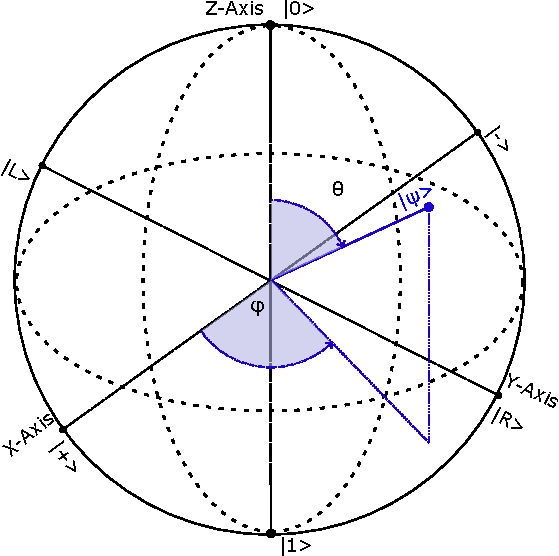
\includegraphics[scale=0.8]{Figures/BlochSphere.pdf}
    \caption{A Bloch Sphere displaying the state $\ket{\psi}$ of a single qubit.}
    \label{fig:bloch_sphere}
\end{figure}
The Pauli matrices represent a rotation\footnote{Pauli matrices are generators of SU(2) group. A complex exponential can be understood as a rotation around a vector $\vec{n}$ where $e^{i\frac{\theta}{2}(\vec{n}\cdot \vec{\sigma})} = \mathbb{I}\cos{\frac{\theta}{2}} + i(\vec{n}\cdot \vec{\sigma})\sin{\frac{\theta}{2}}$.} around a given axis $\{X, Y, Z \}$. The matrix representation is given by,
\begin{align*}
X \equiv \sigma_{x} = \sigma_{1} = 
    \begin{bmatrix}
           0 & 1 \\
           1 & 0 
         \end{bmatrix} \\
Y \equiv \sigma_{y} = \sigma_{2} = 
    \begin{bmatrix}
           0 & -i \\
           i & 0 
         \end{bmatrix} \\ 
Z \equiv \sigma_{z} = \sigma_{3} = 
    \begin{bmatrix}
           1 & 0 \\
           0 & -1 
         \end{bmatrix}
\end{align*}
The eigenvectors of the Pauli matrices are the computational basis vectors,
\begin{align*}
    \Biggl\{\begin{bmatrix}
           1 \\
           0 
         \end{bmatrix}, \begin{bmatrix}
           0 \\
           1 
         \end{bmatrix} \Biggr\}\equiv \{\ket{0}, \ket{1}\} \in Z_{basis} \\
         \Biggl\{\begin{bmatrix}
           \frac{1}{\sqrt{2}} \\
           \frac{1}{\sqrt{2}} 
         \end{bmatrix}, \begin{bmatrix}
           \frac{1}{\sqrt{2}} \\
           -\frac{1}{\sqrt{2}} 
         \end{bmatrix} \Biggr\}\equiv \{\ket{+}, \ket{-}\} \in X_{basis} \\
         \Biggl\{\begin{bmatrix}
           \frac{1}{\sqrt{2}} \\
           \frac{i}{\sqrt{2}} 
         \end{bmatrix}, \begin{bmatrix}
           \frac{1}{\sqrt{2}} \\
           -\frac{i}{\sqrt{2}} 
         \end{bmatrix} \Biggr\}\equiv \{\ket{R}, \ket{L}\} \in Y_{basis}
\end{align*}
In general, we deal with multiple qubits. The basis for an n-qubit system is just the tensor product of n-single-qubit basis.\\
Suppose we have two qubits. Then, the $Z\otimes Z-basis$ is $\{\ket{00},\ket{01},\ket{10},\ket{11}\}$ and the state of a two-qubit system is described by the linear combination,
\begin{equation}
    \ket{\psi} = \alpha_{00}\ket{00} +\alpha_{01}\ket{01} +\alpha_{10}\ket{10} +\alpha_{11}\ket{11}
\end{equation}
where $\|\alpha_{00}\|^{2} + \|\alpha_{01}\|^{2} + \|\alpha_{10}\|^{2} + \|\alpha_{11}\|^{2} = 1$, i.e., the state is normalized.\\
The normalization condition for an n-qubit system can be written as
\begin{equation}
\sum_{x\in \{0,1\}^{n}}\|\alpha_{x}\|^{2} = 1
\end{equation}
Where the expression $x \in \{0,1\}^{n}$ indicates all the possible tensor product combinations of the n-single-qubit states. These combinations form a basis for the n-qubit system.
%%%%%%%%%%%%%%%%%%%%%%%%%%%%%%%%%%%%%%%%%%%%%%%%%%%%%%%%%%%%%%%%%%%%%%%%%%%%%%%%%%%%%%%%%%%%%%%%%%%%%%%%%%
%     A.4 MEASUREMENTS AND OPERATORS
%%%%%%%%%%%%%%%%%%%%%%%%%%%%%%%%%%%%%%%%%%%%%%%%%%%%%%%%%%%%%%%%%%%%%%%%%%%%%%%%%%%%%%%%%%%%%%%%%%%%%%%%%%
\section{Measurements and Operators}
Quantum mechanics makes predictions about microscopic objects taking into account their statistics\footnote{Measurements in an ensemble of equally prepared states gives quantities distributed around a mean value with a given frequency.}. The predictions have implications for the macroscopic world. In classical computing a system is mostly unaltered by tiny interactions such as light or heat. However, in quantum computing this environment noise is quite important as it modify the state of the system. This noise is a doubled-edged sword as it can be used to modify intentionally the state of a quantum system.
\begin{definition}[Operator]
    An operator $\hat{A}$ is a linear map between Hilbert spaces that satisfy,
    \begin{equation}
        \braket{\hat{A}^{\dagger}\psi|\varphi} = \braket{\psi|\hat{A}\varphi} \forall \psi,\varphi \in \mathbb{H}
    \end{equation}
    where $\hat{A}$ admit a matrix representation and "$\dagger$" means transpose conjugate
\end{definition}
\begin{corollary}
    Given an operator $\hat{A}$, on a finite Hilbert space, the operator is said to be Hermitian if
    \begin{equation}
        \hat{A}^{\dagger} = \hat{A}
    \end{equation}
    Hermitian operators play an important role in quantum physics because their eigenvalues are real and represent measurable physical quantities.
\end{corollary}
\begin{definition}[Observable]
    Given the state of a system $\ket{\psi}$, an \textit{observable} -- represented with an operator $\hat{A}$ -- is the physical quantity we can measure associated with the Hermitian operator $\hat{A}$. The possible observables of an operator are its eigenvalues.
\end{definition}
As an example consider the \textit{Hamiltonian} of a system, $\hat{\mathcal{H}}$. For the present work, the Hamiltonian of a system represents the total energy of the system. So, the associated eigenvalues are the eigenenergies of the system.  
\begin{definition}[Unitary Operator]
    An operator U on $\mathbb{H}$ is unitary if
    \begin{equation}
        U^{\dagger}U =\mathbb{I}
    \end{equation}
where $\mathbb{I}$ is the identity operator.
\end{definition}
\begin{definition}[Expectation Value]
    The expectation value, $<\cdot>$, of an observable is the mean value we get after a sequence of measurements of that observable in an ensemble of equally prepared states.
        Mathematically,
    \begin{equation}
        \langle\hat{A}\rangle_{\ket{\psi}} := \braket{\psi |\hat{A}| \psi}
    \end{equation}
\end{definition}

We can measure a classical bit to check if it is in the state 0 or 1. However, when we measure -- in the Z-basis -- a quantum bit we do not get the parameters $\alpha, \beta$ that describe the qubit state. Instead, we get either $\ket{0}$ or $\ket{1}$ with probabilities $\|\alpha\|^{2}$ and $\|\beta\|^{2}$ respectively. The logic of classical computing is Boolean, this means that if the system is not in the state 0 it must be in state 1. In quantum computing, if the system is not in the state 0 it does not have to be in state 1.   

In a measurement, the general state of the qubit collapses to one of the states of the basis we are using to measure. After this measurement the state of our qubit is fixed and successive measurements will give the same state with probability 1, i.e., measurements collapse a qubit into one of the basis states destroying superposition.\\
Quoting Nielsen and Chuang\,\cite{Nielsen2010QuantumInformation},
\begin{displayquote}
\textit{This dichotomy between the unobservable state of a qubit and the observations we can make lies at the heart of quantum computation and quantum information.}
\end{displayquote}
%%%%%%%%%%%%%%%%%%%%%%%%%%%%%%%%%%%%%%%%%%%%%%%%%%%%%%%%%%%%%%%%%%%%%%%%%%%%%%%%%%%%%%%%%%%%%%%%%%%%%%%%%%
%     A.5 SCHRODINGER EQUATION
%%%%%%%%%%%%%%%%%%%%%%%%%%%%%%%%%%%%%%%%%%%%%%%%%%%%%%%%%%%%%%%%%%%%%%%%%%%%%%%%%%%%%%%%%%%%%%%%%%%%%%%%%%
\section{Schrödinger Equation}
One of the paradigms of universal quantum computing is the gate model. This approach substitutes classical logic gates -- such as OR, XOR, AND or NOT -- by its quantum analog. These quantum gates are represented by unitary matrices, so that the inner product is preserved.\\
Equivalently, a quantum gate is represented by a complex exponential of the form\footnote{Where $\hbar$ is the reduced Planck constant.} $\exp\left(i\hat{\mathcal{H}}t / \hbar\right)$ where a given Hamiltonian, $\mathcal{H}$ -- controlled by external fields such as magnetic fields -- leads the evolution of the qubit in such a way that the associated matrix of the complex exponential -- that admit a series expansion -- match the matrix representation of the quantum gate. \\\\
Precisely, the evolution of a quantum system is goberned by the Schrödinger equation which cannot be derived from first principles, i.e., it is an experimental fact. Mathematically, it can be expressed as
\begin{equation}
    \hat{\mathcal{H}}\ket{\psi(t)} = i\hbar \frac{\partial}{\partial t}\ket{\psi(t)}
\end{equation}
where $\hat{\mathcal{H}}$ is the Hamiltonian operator, $\hbar$ is the reduced Planck constant and $\ket{\psi(t)}$ represents the state of a system.\footnote{Remember that in Quantum Physics time does not have an operator so it is not an observable.} and $\ket{\psi(t)}$ represent the state of a system.\\
The Schrödinger equation governs the time evolution of a quantum system. It plays the same role that Newton's equations do in classical mechanics.
%%%%%%%%%%%%%%%%%%%%%%%%%%%%%%%%%%%%%%%%%%%%%%%%%%%%%%%%%%%%%%%%%%%%%%%%%%%%%%%%%%%%%%%%%%%%%%%%%%%%%%%%%%
%     A.6 SPEED-UP ADVANTAGE
%%%%%%%%%%%%%%%%%%%%%%%%%%%%%%%%%%%%%%%%%%%%%%%%%%%%%%%%%%%%%%%%%%%%%%%%%%%%%%%%%%%%%%%%%%%%%%%%%%%%%%%%%%
\section{Speed-up advantage}
We end up this appendix by discussing the main features of quantum behavior that speed-up the algorithms versus its classical approach.\\\\
The main power of quantum computers underlies in three properties,
\begin{itemize}
    \item \textbf{Superposition:} A qubit can be a in a linear combination of states. We can build quantum algorithms that cross out those terms that are not interesting for us and increase the amplitudes of the ones we are interested in.
    \item \textbf{Entanglement:} An entangled state is a state that cannot be written in term of the tensor product of pure states. Entangled states store information exponentially instead of linearly (as classical computing does). As an example, suppose we have the following two-qubit state, called \textit{Bell state}
\begin{equation}
    \ket{\psi} = \frac{1}{\sqrt{2}}\left(\ket{00} + \ket{11}\right)
\end{equation}
If we measure the first qubit in the Z-basis, we can get either the state $\ket{0}$ or $\ket{1}$. We can see that both qubits are entangled in the sense that knowing the state of the first qubit allows us to determine the state of the second qubit. In this case, if the first qubit measurement is $\ket{0}$ we know that the second qubit must be in state $\ket{0}$.\footnote{Einstein termed this effect \emph{spooky action at a distance} in an attempt to ridicule quantum mechanics.}  
    \item \textbf{Parallelism:} A quantum memory register can exist in a superposition of states. If we perform an operation on this quantum register, this operation is applied to all states of that superposition. Notice that we have applied an operation to all the states in that superposition by performing the function just once.
\end{itemize}
Despite the advantage of using quantum computing with respect to classical computing has been proven theorically for some specific problems, see Ref. \cite{Grover19961996Search}, the real world problems are yet far away from being addressed fully by quantum computing\footnote{Nowadays, the hardware is not mature enough for real world industry problems.}. The best we can do nowadays is to solve problems by splitting them into a quantum part that can be done by a quantum computer and a classical part that is solved by using an HPC.
%%%%%%%%%%%%%%%%%%%%%%%%%%%%%%%%%%%%%%%%%%%%%%%%%%%%%%%%%%%%%%%%%%%%%%%%%%%%%%%%%%%%%%%%%%%%%%%%%%%%%%%%%%
%     A.6.1 Grover's Algorithm
%%%%%%%%%%%%%%%%%%%%%%%%%%%%%%%%%%%%%%%%%%%%%%%%%%%%%%%%%%%%%%%%%%%%%%%%%%%%%%%%%%%%%%%%%%%%%%%%%%%%%%%%%%
\subsection{Grover's Algorithm}
In this section we show the advantages of quantum computing by considering a specific example, that of Grover's algorithm.\\
Grover's algorithm is a search algorithm that uses qubits in superposition adjusting their phases to make the computations by quantum parallelism. Given a table with a number of items \textit{N}, we are interested in a particular item $\omega$. The best known classical algorithm can solve the problem in $O(N)$ complexity, which means that in the worst case a classical algorithm has to check each entry of the data-set until finding the item $\omega$ in the last query. Grover's algorithm can solve the problem in $\sim$ $O(\sqrt{N})$ complexity\footnote{This is a lower bound but in some cases the speed up could be better as it happens with the two-qubit system.}, which represent a quadratic speed up compared with the classical approach, i.e., after $\sqrt{N}$ evaluations it is guaranteed to provide the desired state.
\begin{figure}[h]
    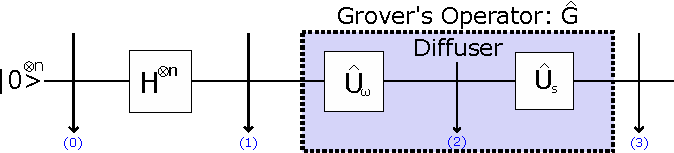
\includegraphics[width=\textwidth]{Figures/Grover_Circuit.pdf}
    \caption{Circuit scheme of Grover's algorithm for an n-qubit system.}
    \label{fig:Grover_circuit}
\end{figure}
\subsubsection{Grover's Algorithm steps for a two-qubit system ($N=4$)}
In this section we show what is the state of the system at each step -- after the application of the quantum gates -- and a geometrical representation based on Ref. \cite{Lavor2008Search} and \textbf{REF}.\\
As an example consider the following table,
\begin{table}[h]
\centering
\label{tab:GroverSearch}
\begin{tabular}{ c | c | c | c | c }
  \hline			
  Binary Index & 00 & 01 & 10 & 11 \\
    \hline		
  Item & 0 & 1 & 2 & 3 \\
  \hline  
\end{tabular}
\caption{Grover's search example. Different items described by its binary expansion.}
\end{table}
and suppose we want to find the item 2, where the index -- binary expansion of decimal index starting from zero -- represents the eigenstate of the system we are looking for. Then, if we are interested in finding the item 2, we are looking for the eigenstate $\ket{\omega} = \ket{10}$.\\
\textbf{(0). Initialized single qubit states:} All the qubits are initialized at $\ket{0}$ so the state of the system is given by the tensor product of the qubits,
\begin{equation}
    \ket{\psi_{0}} = \ket{0}\otimes \ket{0} = \ket{00}
\end{equation}
\textbf{(1). Equiprobability:} Apply a Hadamard gate to each qubit so we create a configuration of equiprobable states\footnote{At the beginning we do not have a good guess of where the item can be so each possibility is equally probable.},
\begin{equation}
    \ket{\psi_{1}} = \hat{H}^{\otimes 2}\ket{00} = \frac{1}{\sqrt{N}}\sum_{x \in \{0,1\}^{2}}\ket{x} \equiv \ket{s}
\end{equation}
 One can label the states using decimal notation, $i = 0 ,\ldots, 2^{n} -1$, where $n$ is the number of qubits.\\
For a two-qubit system,
\begin{equation}
   \{\ket{x}\} = \{\ket{00},\ket{01},\ket{10},\ket{11}\} \equiv \{\ket{0},\ket{1},\ket{2},\ket{3}\} = \{\ket{i}\}
\end{equation}
Therefore, we can re-write the state $\ket{s}$ as
\begin{equation}
    \ket{s} = \frac{1}{\sqrt{N}}\ket{\omega} + \frac{1}{\sqrt{N}}\sum_{i \neq \omega} \ket{i}
\end{equation}
Due to the orthonormality of the basis, $\ket{\omega}$ is orthogonal to $\sum_{i \neq \omega} \ket{i}$. So, we can write
\begin{equation}
    \ket{s} = \sin{\theta}\ket{\omega} + \cos{\theta}\ket{s'}
\end{equation}
where
\begin{equation}
    \sin{\theta} = \frac{1}{\sqrt{N}}, \quad\quad  \ket{s'} = \frac{1}{\cos{\theta}}\frac{1}{\sqrt{N}}\sum_{i\neq \omega}\ket{i}
\end{equation}
\begin{figure}[H]
\centering
    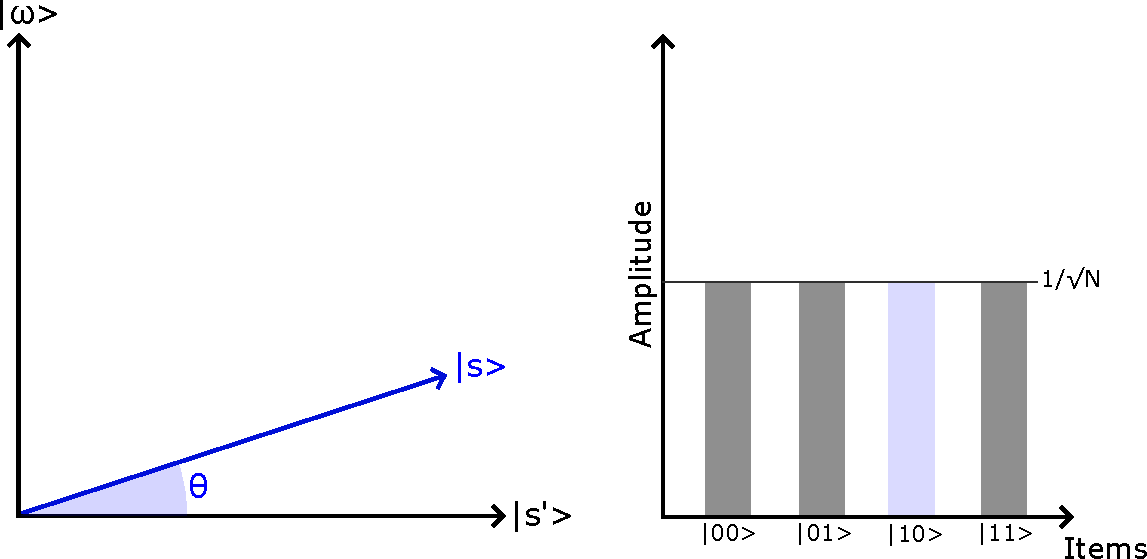
\includegraphics[scale=0.55]{Figures/Grover_Step1.pdf}
    \caption{Amplitude distribution of states after applying a Hadamard gate. The vector $\ket{\omega}$ is our desired state and $\ket{s'}$ is a orthogonal vector. In this way we can write $\ket{s} = \sin{\theta}\ket{\omega} + \cos{\theta}\ket{s'}$.}
    \label{fig:Grover_step1}
\end{figure}
\textbf{(2). Reflection about the state $\ket{s'}$:} Apply an operator $\hat{U}_{\omega}$ defined by
\begin{equation}
     \begin{cases}
       \hat{U}_{\omega}\ket{\omega} = -\ket{\omega} \\
       \hat{U}_{\omega}\ket{i} = \ket{i}, &  \forall \ket{i}\neq \ket{\omega} \\
     \end{cases}
\end{equation}
so the operator can be written as,
\begin{equation}
    \hat{U}_{\omega} = \mathbb{I} - 2\ket{\omega}\bra{\omega}
\end{equation}
Applying the operator to the state $\ket{s}$ yields,
\begin{equation}
    \ket{\psi_{2}} = \hat{U}_{\omega}\ket{s} = \ket{s} -\frac{2}{\sqrt{N}}\ket{\omega} \equiv \ket{\bar{s}}
\end{equation}
\begin{figure}[H]
\centering
    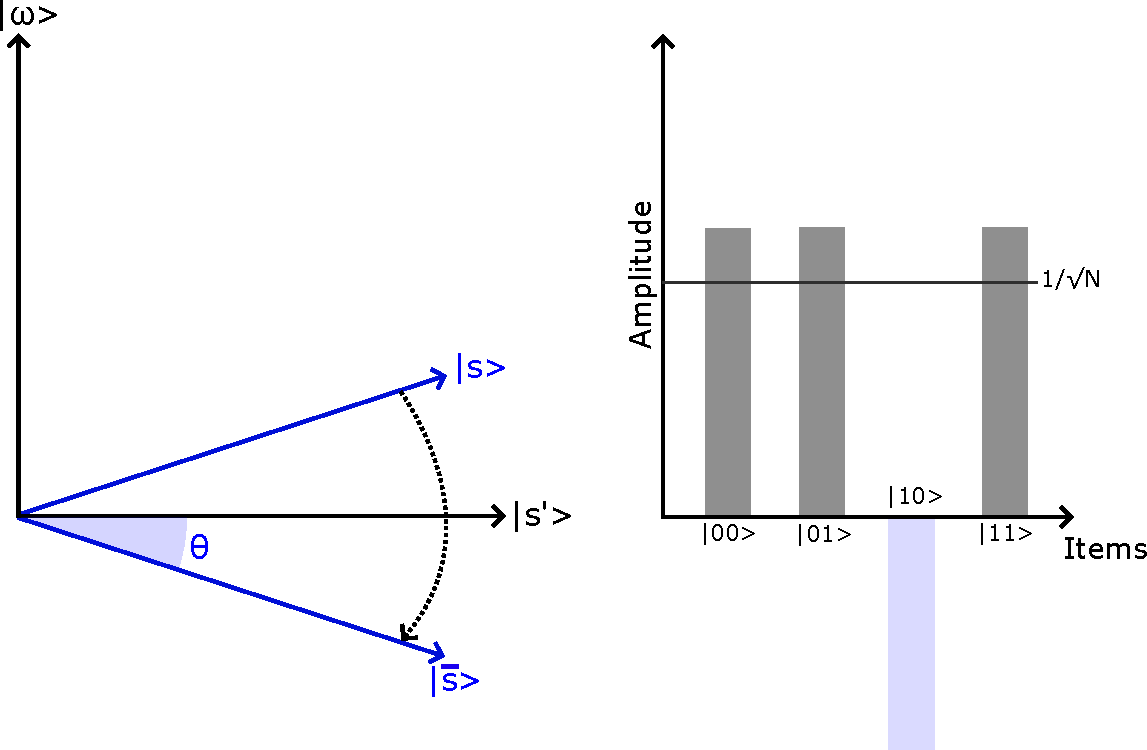
\includegraphics[scale=0.55]{Figures/Grover_Step2.pdf}
    \caption{Amplitude distribution of states after applying a $U_{\omega}$. Notice that we have applied a phase to the state we are looking for. Geometrically this means we have applied a reflection about a state orthonormal to $\ket\omega$.}
    \label{fig:Grover_step2}
\end{figure}
\textbf{(3). Reflection about the state $\ket{s}$:} The operator $\hat{U}_{s}$ is defined as,
\begin{equation}
    \hat{U}_{s} \equiv 2\ket{s}\bra{s} - \mathbb{I}
\end{equation}
Applying the operator to the state of our system yields,
\begin{align*}
    \ket{\psi_{3}} = \hat{U}_{s}\left(\ket{s} -\frac{2}{\sqrt{N}}\ket{\omega}\right) = \left(2\ket{s}\bra{s} - \mathbb{I}\right)\left(\ket{s} - \frac{2}{\sqrt{N}}\ket{\omega}\right) = \frac{N - 4}{N}\ket{s} + \frac{2}{\sqrt{N}}\ket{\omega} \\
    = \frac{1}{N\sqrt{N}} \left[\left(N - 4\right)\sum_{x\neq \omega}\ket{x} + \left(3N-4\right)\ket{\omega}\right] \overset{N=4}{=} \frac{1}{8} \left[0 \cdot \sum_{x\neq \omega}\ket{x} + 8\ket{\omega}\right] = \ket{\omega}
\end{align*}
\begin{figure}[H]
\centering
    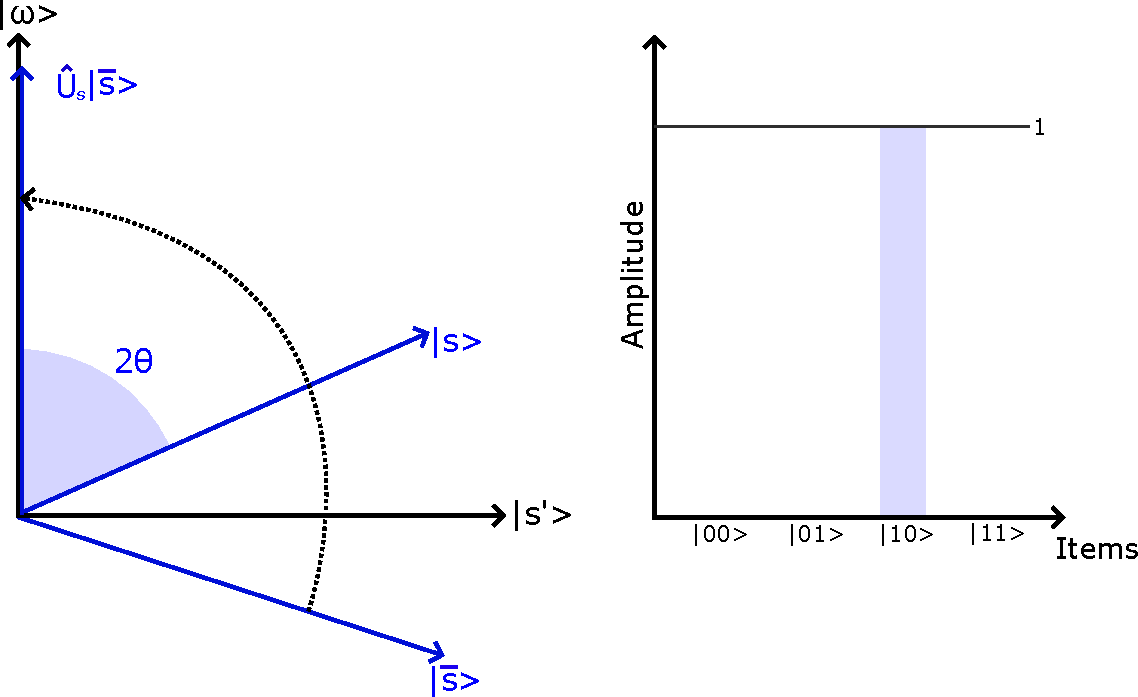
\includegraphics[scale=0.55]{Figures/Grover_Step3.pdf}
    \caption{Amplitude distribution of states after applying $\hat{U}_{s}$. For the case of two qubits, the amplitudes of non-desired states go to zero so we get the desired state $\ket{\omega}$ with a 100\% of probability in an ideal quantum computer. This does not happen if the number of qubits is increased. In that case the amplitudes of non-desired states are reduced compared with the amplitude of the state we are looking for.}
    \label{fig:Grover_step3}
\end{figure}

We have rotated the original state of our system towards the eigenvector $\ket{\omega}$ that represents the item we are looking for in the data-set. The closer\footnote{Notice that the word "close" in this context is referring to the probability of getting the desired state $\ket{\omega}$ when we make a measurement on the system} we want to be to $\ket{\omega}$ the more times we have to repeat \textbf{(2)} and \textbf{(3)}. The quadratic speed up comes from the fact that Grover's algorithm raises the probability amplitude of the item we are looking for by a factor of $\frac{1}{\sqrt{N}}$ .


%Last Comment


% Appendix B

\chapter{Simulated Annealing} % Main appendix title

This appendix justifies the name of the quantum approach we use in the present work -- \textit{Quantum Annealing} (QA) -- to solve \textit{Quadratic Unconstrained Binary Optimization} (QUBO) problems. In the next sections, we show that the expressions we get in the classical approach known as \textit{Simulated Annealing} (SA), have the same functional form as the ones we get with QA \cite{Kadowaki1998QuantumModel}. To do that we are going to develop the solution for a stochastic problem. For a better understanding about stochastic problems see \cite{Schneider2006StochasticOptimization}. 
\label{AppendixB} % For referencing this appendix elsewhere, use \ref{AppendixB}
%%%%%%%%%%%%%%%%%%%%%%%%%%%%%%%%%%%%%%%%%%%%%%%%%%%%%%%%%%%%%%%%%%%%%%%%%%%%%%%%%%%%%%%%%%%%%%%%%%%%%%%%%%
%     B.1 MASTER EQUATION
%%%%%%%%%%%%%%%%%%%%%%%%%%%%%%%%%%%%%%%%%%%%%%%%%%%%%%%%%%%%%%%%%%%%%%%%%%%%%%%%%%%%%%%%%%%%%%%%%%%%%%%%%%
\section{Master Equation}
A master equation is used to characterize the time-evolution of a given system that switches between states according to a transition rate for a given distribution.
\subsection{Discrete Processes}
Suppose we have a space of states $\Gamma = \{\uparrow \uparrow,\downarrow \uparrow,\uparrow \downarrow,\downarrow \downarrow \} \equiv \{1, 2, 3, 4 \}$ and a discrete stochastic process, e.g., $\{X_{t}, t= 0,1,2,...\} \rightarrow \{1,4,2,3,1,..\}$. Furthermore, assume that the actual setting of our system only depends on the previous one, i.e., the probability of being in state \textit{j} at time \textit{t+1}, $X_{t+1}= j$, given that the current state is \textit{i}, $X_{t} = i$, does not depend on previous configurations.\\
Mathematically,
\begin{equation}
\label{eq: MarkovChain}
    P\left(X_{t+1} = j | X_{t} = i\right) = P\left(X_{t+1}=j | X_{t} = i, X_{t-1} =i_{t-1},...,X_{0} = i_{0}\right)
\end{equation}
The equation \ref{eq: MarkovChain} is known as \textbf{Markov chain} condition and the conditional probabilities are named \textit{transition probabilities}.\\
The normalization condition for probabilities is also fulfilled, i.e., starting from a state  \textit{i} any state \textit{j} -- where \textit{j} can be also the current state -- has a transition probability such that
\begin{equation}
    \sum_{j}P\left(X_{t+1} = j | X_{t} = i\right) = 1, \;\; \forall i
\end{equation}
Graphically, this means that the current state of our systems has to be in a given state of $\Gamma$ at any time.
\begin{figure}[H]
    \centering
    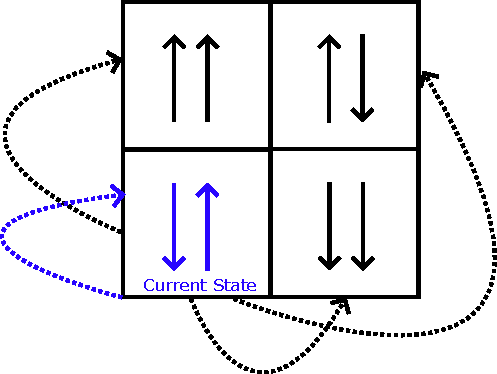
\includegraphics[scale=0.65]{Figures/SA_StateJump.pdf}
    \caption{Stochastic Process for a configuration space $\Gamma$ of four states.}
    \label{fig:SimulatedAnneling_StatesJump}
\end{figure}
\begin{theorem}[Total Probability]
Given an event A in a discrete set of events $\{B_{i}\}$, the probability of occurrence of event A is given by,
\begin{equation}
    P\left(A\right) = \sum_{i}P\left(A|B_{i}\right)P\left(B_{i}\right)
\end{equation}
where $P\left(A|B_{i}\right)$ is the probability of occurrence of event A given that event $B_{i}$ has already happened. 
\end{theorem}
Renaming variables,
\begin{align}
    \label{eq:Renaming1}
    \Pi_{i}(t) \equiv P\left(X_{t} = i\right) \\
    \label{eq:Renaming2}
    p_{i \leftarrow j} := P\left(X_{t+1} = i | X_{t}=j\right)
\end{align}
From equations \ref{eq:Renaming1} and \ref{eq:Renaming2}, we can write,
\begin{align}
        \Pi_{i}(t+1) = p_{i \leftarrow i}\Pi_{i}(t) + \sum_{j \neq i} p_{i \leftarrow j}\Pi_{j}(t) \\ 
        p_{i \leftarrow i} = 1 - \sum_{j\neq i}p_{j \leftarrow i}
\end{align}
Combining the last two equations,
\begin{align}
    \Pi_{i}(t+1) = \left[1 - \sum_{j\neq i}p_{j \leftarrow i}\right]\Pi_{i}(t) + \sum_{j\neq i}p_{i \leftarrow j}\Pi_{j}(t)\\
    \Pi_{i}(t+1) - \Pi_{i}(t) = -\Pi_{i}(t) \sum_{j \neq i}p_{i \leftarrow j} + \sum_{j \neq i} p_{i \leftarrow j}\Pi_{j}(t) \\
    \label{eq: MasterEquationDiscrete}
    d\Pi_{i}(t) := \Pi_{i}(t+1) - \Pi_{i}(t) =  -\Pi_{i}(t) \sum_{j \neq i}p_{i \leftarrow j} + \sum_{j \neq i} p_{i \leftarrow j}\Pi_{j}(t)
\end{align}
we get the master equation of a Markov stochastic discrete process.
\subsection{Continuous Processes}
In case we deal with a continuous process, we need to work with transitions rates defined by,
\begin{equation}
    \mathcal{L}_{i \leftarrow j} = 
    \begin{cases}
    \mathcal{L}_{i \leftarrow j} \;\; i\neq j\\
    -\sum_{k\neq i}\mathcal{L}_{k \leftarrow i} \;\; i = j
    \end{cases}
\end{equation}
so that the master equation can be written as,
\begin{equation}
\label{eq: MasterEquationContinuous}
    \frac{d\Pi_{i}(t)}{dt} = \sum_{j}\mathcal{L}_{i \leftarrow j} \Pi_{j}(t)
\end{equation}
If we know $\Pi_{i}(t_{0})$ we can know the probability at each state. Assume our system has reached the steady state, i.e., $d\Pi_{i}/dt = 0$, which implies,
\begin{equation}
\label{eq: StationaryCondition}
    \Pi_{i}^{\mathrm{eq}} \sum_{j\neq i} \mathcal{L}_{j \leftarrow i} = \sum_{j \neq i}\mathcal{L}_{i \leftarrow j}\Pi_{j}^{\mathrm{eq}} 
\end{equation}
A sufficient but not necessary condition to fulfill \ref{eq: StationaryCondition} is,
\begin{equation}
    \Pi_{i}^{\mathrm{eq}}\mathcal{L}_{j \leftarrow i} = \mathcal{L}_{i \leftarrow j}\Pi_{j}^{\mathrm{eq}} 
\end{equation}
which is known as the \textbf{detailed balanced condition}.\\
The evolution of our system is determined by knowing an initial state and the transition rate expression. Metropolis et al., in connection to statistical mechanics, chose the Boltzmann distribution
\begin{equation}
    \Pi_{i}^{\mathrm{eq}} = \frac{1}{Z}\exp\left(- \frac{\mathcal{H}_{i}}{k_{B}T}\right), \;\;\; Z = \sum_{i}\exp\left(-\frac{\mathcal{H}_{i}}{k_{B}T}\right)
\end{equation}
which implies,
\begin{equation}
    \frac{\mathcal{L}_{j \leftarrow i}}{\mathcal{L}_{i \leftarrow j}} = \exp\left(\frac{\mathcal{H}_{i} - \mathcal{H}_{j}}{k_{B}T}\right)
\end{equation}
The last expression does not define uniquely the transition rate so we need a criterion for that. There are two common criteria:
\begin{itemize}
    \item\textbf{Metropolis criterion:} $\mathcal{L}_{j \leftarrow i} = \min \left[1,\exp\left(\mathcal{H}_{i}-\mathcal{H}_{j}/\left(k_{B}T\right)\right)\right]$. This condition guarantees a transition into states with lower energy without forbidding a transition to higher energy states, where this transition rate depends on the energy difference. 
    \item \textbf{Heat bath criterion:} $\mathcal{L}_{i \leftarrow j} = \frac{\Pi_{j}^{\mathrm{eq}}}{\Pi_{i}^{\mathrm{eq}} + \Pi_{j}^{\mathrm{eq}}} = \left[1 + \exp\left(\frac{\mathcal{H}_{j}- \mathcal{H}_{i}}{k_{B}T}\right)^{-1}\right]$ 
\end{itemize}
 The transition rates do not guarantee the optimal value of our objective function. We must include a time-dependent temperature that guarantees reaching the optimal value when $t \rightarrow \infty$. 
\subsection{Annealing schedules}
The annealing approach considers a temperature that starts from a high value and decreases gradually with time. The dependence of temperature with respect to time $t$ is named annealing schedule. There are many annealing schedules but the most common ones are \footnote{From now on, $k_{B} = 1$.}:
\begin{itemize}
    \item \textbf{Geman-Geman:} This schedule guarantee to reach the absolute minima, see \cite{Geman1984StochasticImages}, in $t \rightarrow \infty$. Mathematically, $T(t) = \frac{a}{b + \log{t}}$
\end{itemize}
Since we do not have infinite time to perform our simulations, we need schedules that are faster despite they do not guarantee convergence to global minimum. 
\begin{itemize}
    \item \textbf{Lineal cooling:} $T(t) = a - bT$ where $a = T_{0}$ -- initial temperature -- and $b \in (0.01,0.2)$.
    \item \textbf{Exponential cooling:} $T(t) = ab^{t}$ where $a = T_{0}$ -- initial temperature -- and $b \in (0.8,0.999)$.
\end{itemize}

%%%%%%%%%%%%%%%%%%%%%%%%%%%%%%%%%%%%%%%%%%%%%%%%%%%%%%%%%%%%%%%%%%%%%%%%%%%%%%%%%%%%%%%%%%%%%%%%%%%%%%%%%%
%     B.2 TSP Example
%%%%%%%%%%%%%%%%%%%%%%%%%%%%%%%%%%%%%%%%%%%%%%%%%%%%%%%%%%%%%%%%%%%%%%%%%%%%%%%%%%%%%%%%%%%%%%%%%%%%%%%%%%
\section{Traveling salesman problem (TSP) by simulated annealing (SA)}
The traveling salesman problem is a NP-hard combinatorial optimization problem. That means it does not have a polynomial time solution. The goal of our traveling salesman is to find the shortest path for visiting all the countries in a list which are represented by nodes of graph. The distance between nodes $i$ and $j$, $D(i,j)$ -- measured in units of length -- is calculated using the Euclidean metric,
\begin{equation}
    D(i,j) \equiv D_{ij}= \sqrt{\left|x_{i} - x_{j}\right|^{2} + \left|y_{i} + y_{j} \right|^{2}} 
\end{equation}
The objective function to minimize for a graph with $n$ nodes can be written as
\begin{equation}
\label{eq:TSP_noconstraints}
    \min_{\vec{x}} f(\vec{x}) = \min_{\vec{x}} \sum_{v} \sum_{u} \sum_{i=0}^{i<n}D_{v,u}x_{v,i}x_{u, i+1}
\end{equation}
where the coefficients $x_{v,i}$ are binary variables that indicates if node $v$ is in the position $i$ of the tour. Furthermore the distance between nodes is symmetric $D_{ij} = D_{ji}$ which is taken into account when creating the matrix $D_{ij}$.\\
The traveling salesman has to visit each node just once in the whole path
\begin{equation}
    \sum_{i}x_{u,i} = 1 \; \forall i
\end{equation}
and each stop of the tour has one node,
\begin{equation}
    \sum_{u}x_{u, i} = 1 \; \forall u
\end{equation}
The constraints can be taken into account in the cost function by using the Lagrange multipliers $\lambda_{i}$, so
\begin{equation}
    \label{eq: ObjectiveMatrixFunction}
   \min_{\vec{x}} f(\vec{x}) = \min_{\vec{x}} \sum_{v} \sum_{u} \sum_{i=0}^{i<n}D_{v,u}x_{v,i}x_{u, i+1} - \sum_{i}\lambda_{i}\left(\sum_{u} x_{u, i} - 1\right)^{2} - \sum_{u}\lambda_{u} \left( \sum_{i}x_{u,i} - 1\right)^{2}
\end{equation}
For simplicity, assume all Lagrange multipliers has the same weight, so \ref{eq: ObjectiveMatrixFunction} is simplified 
\begin{equation}
    \min_{\vec{x}} f(\vec{x}) = \min_{\vec{x}} \sum_{v} \sum_{u} \sum_{i=0}^{i<n}D_{v,u}x_{v,i}x_{u, i+1} - \sum_{i}\left(\sum_{u} x_{u, i} - 1\right)^{2} - \sum_{u}\left( \sum_{i}x_{u,i} - 1\right)^{2} 
\end{equation}
By expanding and dropping constant factors
\begin{align*}
    \min_{\vec{x}} f(\vec{x}) = \min_{\vec{x}} \sum_{v} \sum_{u} \sum_{i=0}^{i<n}D_{v,u}x_{v,i}x_{u, i+1} \\
    -\sum_{i}\left( \sum_{u}x_{u,i}^{2} + 2\sum_{u<v}x_{u,i}x_{v,i} - 2\sum_{u}x_{u,i}\right)  \\
    - \sum_{u}\left( \sum_{i}x_{u,i}^{2} + 2\sum_{i<j}x_{u,i}x_{u,j} - 2\sum_{i}x_{u,i}\right)
\end{align*}
Simplifying last expression
\begin{equation}
    \min_{\vec{x}} \sum_{v} \sum_{u} \sum_{i}D_{v,u}x_{v,i}x_{u, i+1} - 2 \sum_{i}\sum_{u} \left(x_{u,i}^{2} + 2 x_{u,i} \right) - 2 \sum_{i}\sum_{u<v}x_{u,i}x_{v,i}- 2 \sum_{u}\sum_{i<j}x_{u,i}x_{u,j}
\end{equation}
for binary variables it is satisfied $x^{2} = x$
\begin{equation}
       \min_{\vec{x}} \sum_{v} \sum_{u} \sum_{i}D_{v,u}x_{v,i}x_{u, i+1} - 6 \sum_{i}\sum_{u} x_{u,i}^{2} - 2 \sum_{i}\sum_{u<v}x_{u,i}x_{v,i}- 2 \sum_{u}\sum_{i<j}x_{u,i}x_{u,j}
\end{equation}
We can write the problem in matrix form
\begin{equation}
    \min_{X} X^{T} Q X
\end{equation}
where
\begin{equation}
Q_{uv,ij} = 
    \begin{cases}
    -2  & \text{if } u=v \\
    -2  & \text{if } i=j \\
    -6  & \text{if } u=v;i=j \\
    D_{u,v} & \text{other }
    \end{cases}
\end{equation}
This statements differs from the QUBO formulation in the sense we are using a binary matrix $X$ instead of binary vectors.\\\\
If the constraints are taken into account in the loops of our program, then the function to minimize is just \ref{eq:TSP_noconstraints}.
\begin{figure}
    \centering
    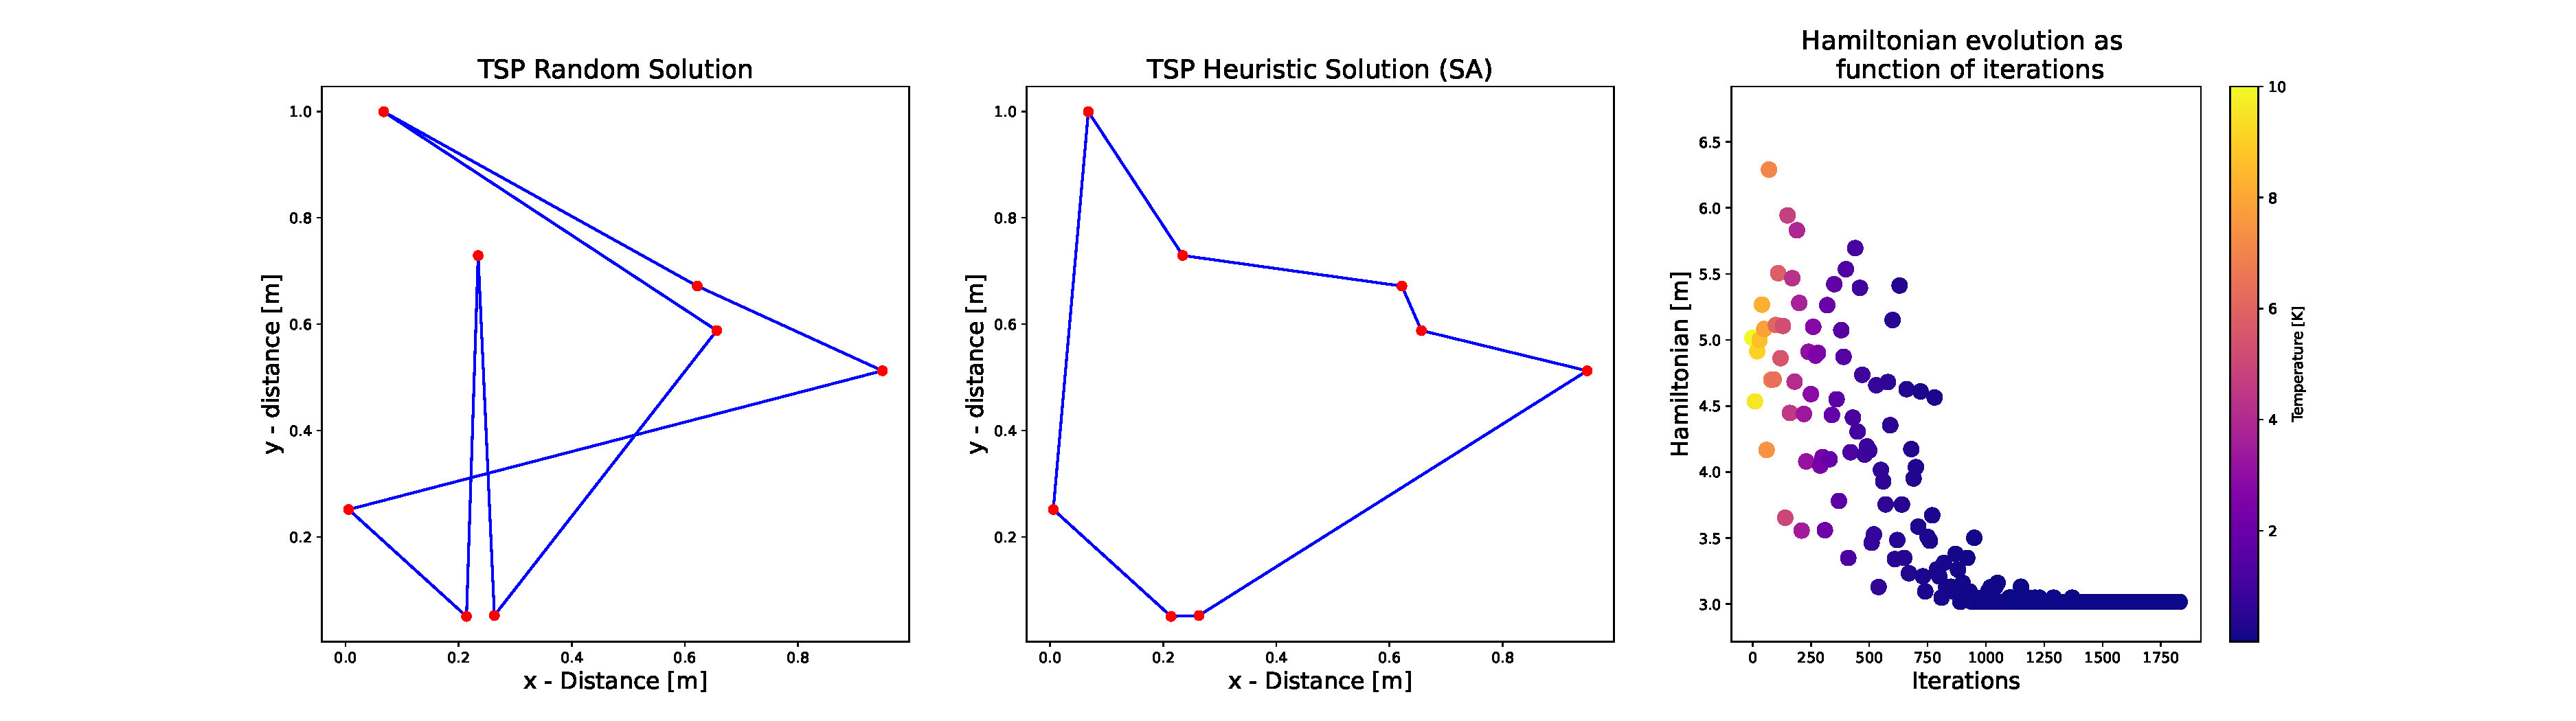
\includegraphics[width=\textwidth]{Figures/TSP_SA.pdf}
    \caption{AGREGAR CAPTION}
    \label{fig:TSP_SA}
\end{figure}


% Appendix C

\chapter{Topology} % Main appendix title

This appendix justifies the name of the quantum approach we use in the present work -- \textit{Quantum Annealing} (QA) -- to solve \textit{Quadratic Unconstrained Binary Optimization} (QUBO) problems. In the next sections, we show that the expressions we get in the classical approach known as \textit{Simulated Annealing} (SA), have the same functional form as the ones we get with QA \cite{Kadowaki1998QuantumModel}. To do that we are going to develop the solution for a stochastic problem. For a better understanding about stochastic problems see \cite{Schneider2006StochasticOptimization}. 
\label{AppendixC} % For referencing this appendix elsewhere, use \ref{AppendixB}
%%%%%%%%%%%%%%%%%%%%%%%%%%%%%%%%%%%%%%%%%%%%%%%%%%%%%%%%%%%%%%%%%%%%%%%%%%%%%%%%%%%%%%%%%%%%%%%%%%%%%%%%%%
%     B.1 MASTER EQUATION
%%%%%%%%%%%%%%%%%%%%%%%%%%%%%%%%%%%%%%%%%%%%%%%%%%%%%%%%%%%%%%%%%%%%%%%%%%%%%%%%%%%%%%%%%%%%%%%%%%%%%%%%%%

% Appendix D

\chapter{Introduction to Oceans} % Main appendix title

This appendix justifies the name of the quantum approach we use in the present work -- \textit{Quantum Anneling} (QA) -- to solve \textit{Quadratic Unconstrained Binary Optimization} (QUBO) problems. In the next sections, we show that the expressions we get in the classical approach known as \textit{Simulated Annealing} (SA), have the same functional form as the ones we get with QA \cite{Kadowaki1998QuantumModel}. To do that we are going to develop the solution for a stochastic problem. For a better understanding about stochastic problems see \cite{Schneider2006StochasticOptimization}. 
\label{AppendixD} % For referencing this appendix elsewhere, use \ref{AppendixB}
%%%%%%%%%%%%%%%%%%%%%%%%%%%%%%%%%%%%%%%%%%%%%%%%%%%%%%%%%%%%%%%%%%%%%%%%%%%%%%%%%%%%%%%%%%%%%%%%%%%%%%%%%%
%     B.1 MASTER EQUATION
%%%%%%%%%%%%%%%%%%%%%%%%%%%%%%%%%%%%%%%%%%%%%%%%%%%%%%%%%%%%%%%%%%%%%%%%%%%%%%%%%%%%%%%%%%%%%%%%%%%%%%%%%%


%\include{Appendices/AppendixC}

%----------------------------------------------------------------------------------------
%	BIBLIOGRAPHY
%----------------------------------------------------------------------------------------

\printbibliography[heading=bibintoc]

%----------------------------------------------------------------------------------------

\end{document}  
